% ****** Start of file apssamp.tex ******
%
%   This file is part of the APS files in the REVTeX 4.1 distribution.
%   Version 4.1r of REVTeX, August 2010
%
%   Copyright (c) 2009, 2010 The American Physical Society.
%
%   See the REVTeX 4 README file for restrictions and more information.
%
% TeX'ing this file requires that you have AMS-LaTeX 2.0 installed
% as well as the rest of the prerequisites for REVTeX 4.1
%
% See the REVTeX 4 README file
% It also requires running BibTeX. The commands are as follows:
%
%  1)  latex apssamp.tex
%  2)  bibtex apssamp
%  3)  latex apssamp.tex
%  4)  latex apssamp.tex
%
\documentclass[%
 reprint,
%superscriptaddress,
%groupedaddress,
%unsortedaddress,
%runinaddress,
%frontmatterverbose,
%preprint,
%showpacs,preprintnumbers,
%nofootinbib,
%nobibnotes,
%bibnotes,
 amsmath,amssymb,
 aps,
%pra,
%prb,
%rmp,
%prstab,
%prstper,
%floatfix,
]{revtex4-1}

\usepackage[caption=false]{subfig}
\usepackage[pass,letterpaper]{geometry}
\usepackage{multirow}
\usepackage{graphicx}% Include figure files
\usepackage{dcolumn}% Align table columns on decimal point
\usepackage{bm}% bold math
\usepackage{longtable}
\usepackage{afterpage}
\usepackage{tabularx}
\usepackage[version=3]{mhchem}
\usepackage[]{SIunits}

% Support for subfigure w/ reference


%\usepackage{hyperref}% add hypertext capabilities
%\usepackage[mathlines]{lineno}% Enable numbering of text and display math
%\linenumbers\relax % Commence numbering lines

%\usepackage{showframe}%Uncomment any one of the following lines to test
%%scale=0.7, marginratio={1:1, 2:3}, ignoreall,% default settings
%%text={7in,10in},centering,
%%margin=1.5in,
%%total={6.5in,8.75in}, top=1.2in, left=0.9in, includefoot,
%%height=10in,a5paper,hmargin={3cm,0.8in},
%]{geometry}

\begin{document}

\preprint{APS/123-QED}

\title{
  Monovacancy Properties From Atomistic Simulations Based on OpenKIM
}% Force line breaks with \\
%\thanks{A footnote to the article title}%

\author{Junhao Li}
  \email{jl2922@cornell.edu}
\author{Matt Bierbaum}
\affiliation{
  Department of Physics and Laboratory of Atomic and Solid State Physics\\
  Cornell University, Ithaca, NY 14853, USA
}
\author{Ryan Elliott}
\author{Ellad Tadmor}
\affiliation{
  Department of Aerospace Engineering and Mechanics\\
  University of Minnesota, Minneapolis, MN 55455, USA
}
\author{James P. Sethna}
  \email{sethna@lassp.cornell.edu}
\affiliation{
  Department of Physics and Laboratory of Atomic and Solid State Physics\\
  Cornell University, Ithaca, NY 14853, USA
}
%\author{Ann Author}
% \altaffiliation[Also at ]{Physics Department, XYZ University.}%Lines break automatically or can be forced with \\
%\author{Second Author}%
% \email{Second.Author@institution.edu}
%\affiliation{%
% Authors' institution and/or address\\
% This line break forced with \textbackslash\textbackslash
%}%
%
%\collaboration{MUSO Collaboration}%\noaffiliation
%
%\author{Charlie Author}
% \homepage{http://www.Second.institution.edu/~Charlie.Author}
%\affiliation{
% Second institution and/or address\\
% This line break forced% with \\
%}%
%\affiliation{
% Third institution, the second for Charlie Author
%}%
%\author{Delta Author}
%\affiliation{%
% Authors' institution and/or address\\
% This line break forced with \textbackslash\textbackslash
%}%
%
%\collaboration{CLEO Collaboration}%\noaffiliation

\date{\today}% It is always \today, today,
             %  but any date may be explicitly specified

\begin{abstract}
In this paper, we describe how we obtain the monovacancy properties for all the elements and all the simple crystal structures with interatomic potential models available on OpenKIM.
The properties we calculated includes the vacancy formation energy (VFE), the vacancy migration energy (VME), the vacancy relaxation volume (VRV), the elastic dipole tensor (EDT), the defect strain tensor (DST), the saddle point elastic dipole tensor (SPEDT), and the saddle point defect strain tensor (SPDST).
The structures we calculated includes sc, fcc, bcc, diamond, and hcp.
These results can provide use information when selecting interatomic models and can also be used with a continuous model to obtain an initial guess for further atomistic simulations.
We also exam how these results depends on each other and on other elemental properties.

%An article usually includes an abstract, a concise summary of the work
%covered at length in the main body of the article.
%\begin{description}
%\item[Usage]
%Secondary publications and information retrieval purposes.
%\item[PACS numbers]
%May be entered using the \verb+\pacs{#1}+ command.
%\item[Structure]
%You may use the \texttt{description} environment to structure your abstract;
%use the optional argument of the \verb+\item+ command to give the category of each item.
%\end{description}
\end{abstract}

%\pacs{Valid PACS appear here}% PACS, the Physics and Astronomy
                             % Classification Scheme.
%\keywords{Suggested keywords}%Use showkeys class option if keyword
                              %display desired
\maketitle

%\tableofcontents

\section{\label{sec:intro}Introduction}

A longtime goal of scientists' is to be able to calculate the properties of materials from their structures accurately and efficiently.
There are several approaches to this problem, including density functional theory (DFT) and atomistic simulation.
DFT has developed rapidly in the recent few decades and achieved decent accuracy for many small-scale systems.
However, in many cases, the size, the complexity, or the timescale we want to simulate, demands a much more efficient method.
And atomistic simulation with good interatomic potentials is one of the methods that can fulfill this demand.

Several different types of interatomic models have been developed over the past few decades, from pairwise models like Lennard-Jones, to those based on cluster functionals, such as embedded-atom method (EAM) \cite{daw1993embedded, daw1984embedded}.
One problem that has hindered the development of atomistic simulation is that the models developed by various researchers are usually presented in different formats, making them difficult to be reused.
The OpenKIM project \cite{bierbaum2014openkim, openkim2016} solves this problem by providing a unified framework for model developers to submit, and for model users to perform atomistic simulations with these models \cite{tadmor2011potential}.
It also hosts a repository of reference data from other sources, such as DFT and experiments, to assess the quality of these models.
% sample elements from the whole periodic table and various structures and find out or discover suitable materials and structures in an automated way, which in the past could only be done with DFT \cite{ceder2010opportunities, zhou2010iron,norskov2009towards} and thus was only applicable for small structures.

In this study, we focus on vacancies.
Finding interatomic models that can accurately describe vacancy effects is extremely beneficial for furthering our understanding and application of materials.
Vacancies are the simplest and the most common defects.
They affect dislocation climbing and creeping \cite{weertman1955theory}, mediate the diffusion of substitutional defects \cite{fahey1989point}, and are the dominant flow mechanism under external fields, such as gravity \cite{sethna2014flow}.
Also, some scientists are proposing using \ce{^{28}Si} for a new kilogram definition \cite{andreas2011counting}, and how to obtain the vacancy concentration accurately will be a crucial part of this work.

In order to assess how each interatomic potential model performs in vacancy-related simulations, we calculated the monovacancy properties for all the elements and all the simple crystal structures with interatomic potential models available on OpenKIM.
The properties we calculated includes the vacancy formation energy (VFE), the vacancy migration energy (VME), the vacancy relaxation volume (VRV), the elastic dipole tensor (EDT), the defect strain tensor (DST), the saddle point elastic dipole tensor (SPEDT), and the saddle point defect strain tensor (SPDST).
Appendix~\ref{app:definition} provides a brief description to these quantities.
Sec.~\ref{sec:method} describes how we calculate these quantities.
The structures we calculated includes sc, fcc, bcc, diamond, and hcp.
These results can be compared with data from other sources, such as density function theory (DFT), quantum monte carlo (QMC), and experiments, and provide use information for selecting interatomic models when performing vacancy-related simulations.
They can also be used with continuous models to obtain an initial guess for further atomistic simulations \cite{bozhevolnyi2001multiple}.

We compared our VFE and VME results to DFT calculations and experiments for fcc and hcp structures \cite{angsten2014elemental}.
We found that EAM potential models, in general, provide results closer to these reference data then other models, especially for transition metals.

In addition, we explored how these properties relate to each other, and to other elemental properties, such as the cohesive energy and the bulk modulus.

The paper is organized as follows.
In Sec.~\ref{sec:method} we describe the algorithm used for calculating the monovacancy properties.
In Sec.~\ref{sec:results} we show the plots of our results, compare them with the reference data, and explore how they relate to each other and to other elemental properties.
Sec.~\ref{sec:conclusion} concludes this paper.
And Appendix~\ref{app:results} list the scripts used for obtaining the data from OpenKIM.

\section{\label{sec:method}Methodology}

In this section, we explain how we calculated the monovacancy properties, including the vacancy formation energy (VFE), the vacancy migration energy (VME), the vacancy relaxation volume (VRV), the elastic dipole tensor (EDT), the defect strain tensor (DST), the saddle point elastic dipole tensor (SPEDT), and the saddle point defect strain tensor (SPDST).
For a brief description of these quantities, see Appendix~\ref{app:definition} and the OpenKIM website \url{https://openkim.org/properties}.

The calculation is based on OpenKIM and the Atomic Simulation Environment (ASE) \cite{bahn2002object}.

The free energy per unit volume of a crystal can be described by the following equation
\begin{equation}\label{eq:f}
f = f_0 + n_dE_d + \frac{1}{2}n_d^2E_{dd} + \frac{1}{2}C_{ijkl}\epsilon_{ij}\epsilon_{kl} - n_d\epsilon_{ij}G_{ij}
\end{equation}
where $n_d$ is the defect concentration, $\epsilon_{ij}$ is the bulk strain, $E_d$ is the vacancy formation energy, $E_dd$ describes the energy from defect interaction, $C_{ijkl}$ is the elastic stiffness tensor, and $G_{ij}$ is the elastic dipole tensor \cite{freedman2009elastic}.
$f_0$ is the chemical potential.
Suppose $n$ is the number of atoms per unit volume and $E_0$ is the energy per atom corresponding to a perfect crystal (the reservoir), then $f_0 = (n - n_d) E_{0}$.

The negative direvative of $f$ with respect to $n_d$ under zero strain gives vacancy formation energy, VFE
\begin{equation}
  \label{eq:VFE0}
  \mathit{VFE} = E_d = \left.\frac{\partial f}{\partial n_d}\right|_{\epsilon = 0} + E_{0} - n_d E_{dd}
\end{equation}
For a supercell of volume $V_0$ with a monovacancy, Eq.~\ref{eq:VFE0} is equivalent to
\begin{equation}
  (E_{V_0, d} - E_{V_0}) + E_{0} = \mathit{VFE} + \frac{E_{dd}}{V_0}
\end{equation}
Here $E_{V_0, d}$ and $E_{V_0}$ are the free energy of the supercell with and withouth the defect, respectively.
Since $E_{dd}$ is unknown, we obtained VFE through extrapolation.
The uncertainty of this value is the combination of the uncertainty from extrapolation and the uncertainty from atomistic relaxation.

The negative derivative of $f$ with respect to strain gives the stress
\begin{equation}
  \label{eq:stress}
  \sigma_{ij} = -\frac{\partial f}{\partial \epsilon_{ij}}
  = -C_{ijkl}\epsilon_{kl} + n_dG_{ij} - \frac{1}{2}n_d^2\frac{\partial E_{dd}}{\partial \epsilon_{ij}}
\end{equation}
And the derivative of $\sigma_{ij}$ with respect to $n_d$ with fixed strain $\epsilon_0$ gives elastic dipole tensor, EDT ($G_{ij}$)
\begin{equation}
  \label{eq:EDT}
  G_{ij} = \left.\frac{\partial \sigma_{ij}}{\partial n_d}\right|_{\epsilon = \epsilon_0}
  + n_d \left.\frac{\partial E_{dd}}{\partial \epsilon_{ij}}\right|_{\epsilon = \epsilon_0}
\end{equation}
We obtained the value and the uncertainty of EDT through extrapolating the results of supercells as what we did for VFE.

The defect strain tensor, DST ($\Lambda_{ij}$) is obtained by
\begin{equation}
  \label{eq:DST}
  \Lambda_{ij} = S_{ijkl} G_{kl}
\end{equation}
where $S_{ijkl}$ is the elastic compliance tensor, which is the inverse of the elastic stiffness tensor.

The relaxation volume, VRV, is the trace of the defect strain tensor.

For vacancy migration, we used nudged elastic band method to obtain the migration path.
The vacancy migration energy, VME, is calculated as the energy different between the energy saddle point configuration along the migration path and the initial configuration.
We obtain the elastic dipole tensor and the defect strain tensor similarly with the saddle point configuration.
Since the configuration of the saddle point is still a monovacancy, the quantities scale in the same way as in the static case with respect to the number of atoms.

\begin{figure}
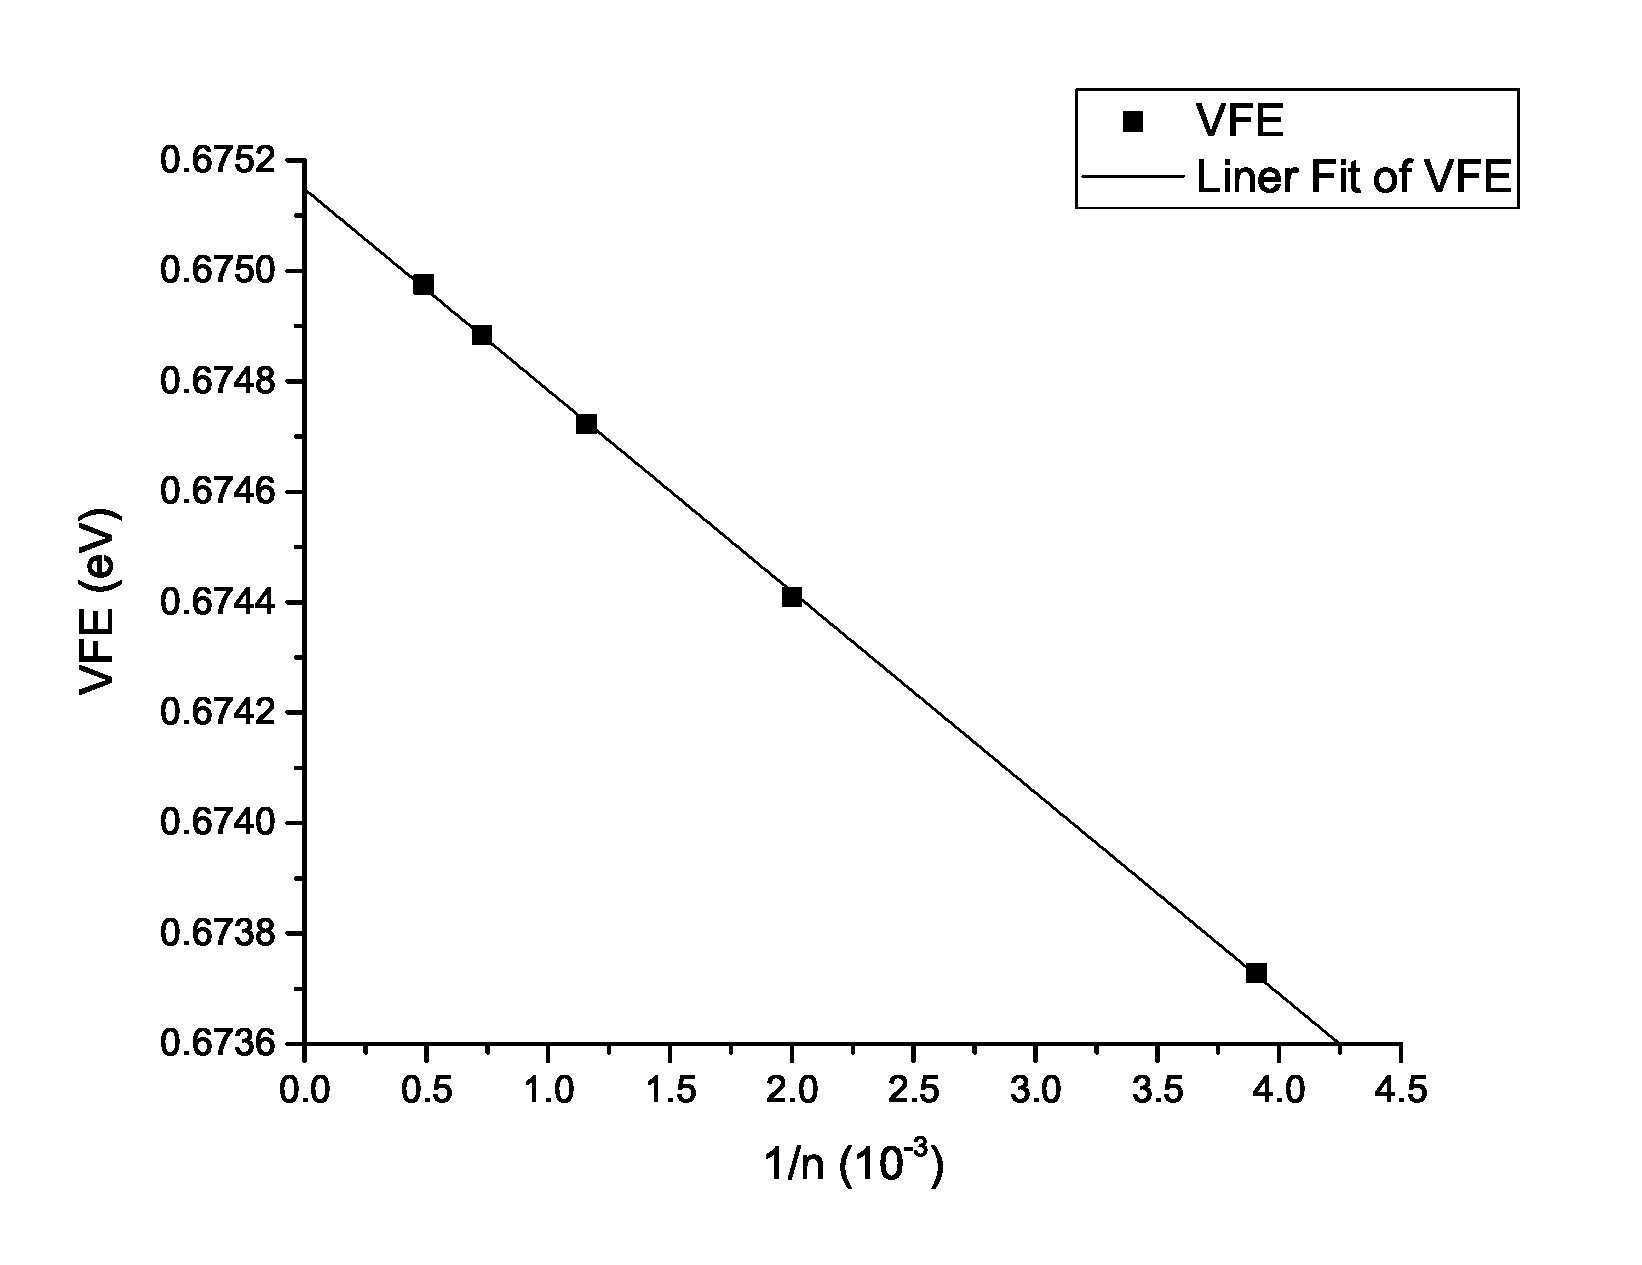
\includegraphics[width=0.5\textwidth]{AlMishinVFEFitting}% Here is how to import EPS art
\caption{\label{fig:VFEFitting}
  Monovacancy formation energy (VFE) versus the inverse of the number of atoms ($n$) in a supercell, calculated with the embedded atom model (EAM) of aluminum from Mishin and Farkas \cite{mishin1999interatomic}.
  As we can see from this plot, there is a strong linear correlation between VFE and $1/n$.
  The adjusted R-square of the linear fitting is 0.99978.
  The intercept of the fitted line corresponds to VFE of the dilute limit $\unit{0.67515(1)}{\electronvolt}$.
}
\end{figure}

The code that implements the whole algorithm is available in the OpenKIM repository \cite{openkim2016}, id: 554849987965.
%
%
% We first obtain the lattice constants through energy minimization, and then use this value to build several periodically repeated supercells of different sizes.
% For each supercell, we use the following algorithm to obtain the desired properties:
%
% \begin{enumerate}
%  \item Obtain the potential energy and volume of this supercell, $E_0$ and $V_0$.
%  \item Remove an atom, relax the positions of the other atoms (keep the size of the supercell fixed) and obtain the new potential energy, $E_1$.
%  \item Calculate the vacancy formation energy by:
%  \begin{equation}
%  \label{eq:vfecalc}
%  \mathit{VFE} = E_1 - E_0 \times \frac{n - 1}{n}
%  \end{equation}
%  where $n$ is the number of atoms in the original supercell.
%  \item Move one atom to the vacant site from the nearest neighbors and use the nudged elastic band (NEB) method to obtain the saddle point energy, $E_2$.
%  \item Calculate the vacancy migration energy by:
%  \begin{equation}
%  \label{eq:vmecalc}
%  \mathit{VME} = E_2 - E_1
%  \end{equation}
%  \item Relax the size of the supercell and obtain the relaxation volume.
% \end{enumerate}
%
% Finally, we extrapolate these results to get the dilute limit.
% The extrapolation is based on the elastic theory \cite{landau2013course}, according to which all the quantities that we are interested in scale approximately as
% \begin{equation}
% \label{eq:extrapolation}
% A_0 + \frac{A_3}{n}
% \end{equation}
% where $n$ is the number of atoms in a supercell \cite{freysoldt2014first}, and $A_0$ and $A_3$ are the constants to be determined.
% $A_0$ is the dilute limit we want.
%
% We can prove this scaling relationship as follows:
% first of all, $n\propto R^3$, where $R$ is the size of the supercell, so Eq.~(\ref{eq:extrapolation}) is equivalent to $A_0+A_3/R^3$.
% For simplicity, we ignore anisotropy and nonlinearity, and consider the supercell with a vacancy as a hollow sphere.
% According to the elastic theory, the displacement vector of a hollow sphere of external and internal radii $R_1$ and $R_2$ with a pressure $p_1$ inside and $p_2$ outside is $\vec{u} = \left(ar + b / r^2\right)\hat{r}$, where
% \begin{align}
% a &= \frac{p_1R_1^3-p_2R_2^3}{R_2^3-R_1^3}\cdot\frac{1-2\sigma}{E}\\
% b &= \frac{R_1^3R_2^3(p_1-p_2)}{R_2^3-R_1^3}\cdot\frac{1+\sigma}{2E}
% \end{align}
% Here $\sigma$ is the Poisson's ratio, $E$ is the Young's modulus, $p_2=0$, and, for VRV, $r=R_2$. Hence, we can get the $r$ component of $\vec{u}$
% \begin{equation}
% \label{eq:ur}
% u_r = \frac{p_1R_1^3}{R_2^2}\cdot\frac{3\left(1-\sigma\right)}{2E}\left(1+\frac{R_1^3}{R_2^3}+O\left(\frac{1}{R_2^6}\right)\right)
% \end{equation}
% Therefore, the vacancy relaxation volume
% \begin{equation}
% \label{eq:VRVProof}
% \begin{split}
% \mathit{VRV} & = \frac{4}{3}\pi\left(R_2^3-(R_2-u_r)^3\right)\\
%  & = 4\pi C_0\left(1 + \frac{R_1^3-C_0}{R_2^3} + O\left(\frac{1}{R_2^6}\right)\right)
% \end{split}
% \end{equation}
% Here $C_0 = 3p_1R_1^3(1-\sigma)/2E$ is a constant.
% Eq.~(\ref{eq:VRVProof}) indicates that VRV satisfies Eq.~(\ref{eq:extrapolation}).
%
% The strain and the stress of the hollow sphere are
% \begin{align}
% u_{rr} &= a - 2b/r^3\\
% u_{\theta\theta} = u_{\phi\phi} &= a + b/r^3\\
% \sigma_{rr} &= \frac{pR_1^3}{R_2^3-R_1^3}\cdot \left(1-\frac{R_2^3}{r^3}\right)\\
% \sigma_{\theta\theta}=\sigma_{\phi\phi} &= \frac{p_1R_1^3}{R_2^3-R_1^3}\cdot\left(1+\frac{R_2^3}{r^3}\right)
% \end{align}
% From these we can obtain the vacancy formation energy
% \begin{equation}
% \label{eq:VFEProof}
% \begin{split}
% \mathit{VFE} & = \iiint_V \frac{1}{2} \left(u_{rr}\sigma_{rr} + u_{\theta\theta}\sigma_{\theta\theta} + u_{\phi\phi}\sigma_{\phi\phi}\right) dV\\
%  & = 4C_1(1+\sigma)
%  + 2C_1 C_2 \cdot\frac{R_1^3}{R_2^3}
%  + O\left(\frac{1}{R_2^6}\right)
% \end{split}
% \end{equation}
% where $C_1=p_1^2\pi R_1^3/(3E)$ and $C_2 = 5-4\sigma+(6\sigma-3) \log\left(R_1/R_2\right)$.
% This proves that VFE scales approximately as Eq.~(\ref{eq:extrapolation}).
%
% Note that, for efficiency, our calculation of VFE is performed with a fixed-size supercell, not a stress-free one.
% This will not affect the results, because the difference between the results from the two different boundary conditions is
% \begin{equation}
% \Delta E=\int pdV=\int B \frac{V-V_0}{V_0}dV\propto\frac{(V-V_0)^2}{V_0}
% \end{equation}
% where the numerator is $\mathit{VRV}^2=16\pi C_0^2+O(R_2^{-3})$, and the denominator is proportional to $R_2^3$.
% This means $\Delta E$ also scales as $1/R_2^3$.
%
% VME is the energy difference between two configurations:
% a crystal with a monovacancy, and a crystal with two monovacancies adjacent to each other and an extra atom somewhere between the two vacant sites.
% The energy of the first configuration has just been proved to scale as Eq.~(\ref{eq:extrapolation}).
% The second configuration can be considered as a superposition of three states:
% two states correspond to the initial and final states of the migration, and the third one corresponds to the saddle point but with the two vacant sites filled up.
% The proof of VFE can be applied directly to each of these states and give similar $R_2$ dependencies.
% Therefore, VME also satisfies Eq.~(\ref{eq:extrapolation}).
%
% Fig.~\ref{fig:VFEFitting} is a plot of VFE versus $1/n$, calculated with the EAM model of aluminum from Mishin and Farkas \cite{mishin1999interatomic}.
% In this case, $A_0 = \unit{0.67515(1)}{\electronvolt}$ and $A_3 = \unit{-0.3644(27)}{\electronvolt}$, which implies that the monovacancy formation energy is \unit{0.67515(1)}{\electronvolt}.
% The linear relationship shown in this figure and the adjusted R-square of 0.99978 in the fitting validate our extrapolation.

% \begin{figure}
% 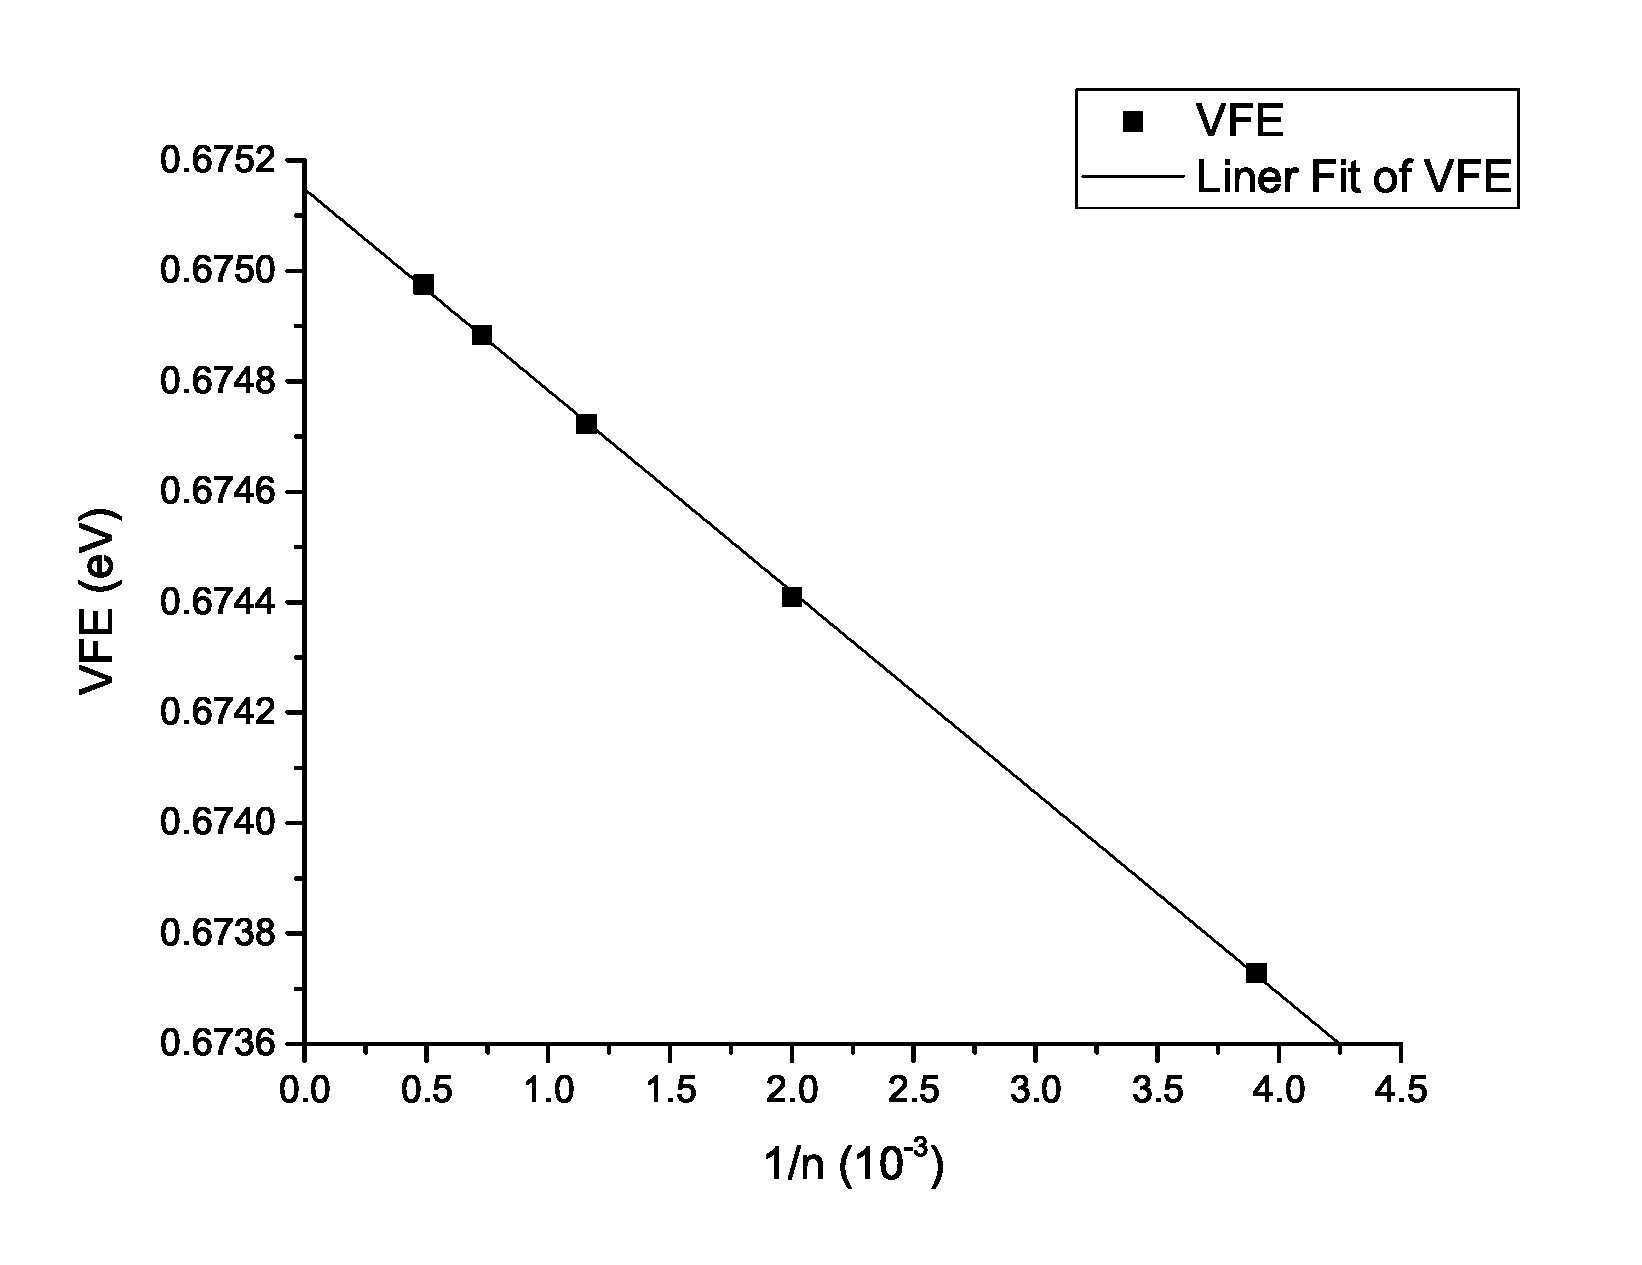
\includegraphics[width=0.5\textwidth]{AlMishinVFEFitting}% Here is how to import EPS art
% \caption{\label{fig:VFEFitting}
%   Monovacancy formation energy (VFE) versus the inverse of the number of atoms ($n$) in a supercell, calculated with the embedded atom model (EAM) of aluminum from Mishin and Farkas \cite{mishin1999interatomic}.
%   As we can see from this plot, there is a strong linear correlation between VFE and $1/n$.
%   The adjusted R-square of the linear fitting is 0.99978.
%   The intercept of the fitted line corresponds to VFE of the dilute limit $\unit{0.67515(1)}{\electronvolt}$.
% }
% \end{figure}
%
% The code that implements the whole algorithm is available in the OpenKIM repository \cite{openkim2016}, id: 554849987965.

\section{\label{sec:results}Results and Discussion}

\subsection{\label{sec:calcvsref}Calculated Results Versus Reference Data}

All the results calculated in this work are available in the OpenKIM repository \cite{openkim2016}.
In Appendix~\ref{app:data}, we list the scripts that can automatically retrieve these results through OpenKIM Query, the data querying API provided by OpenKIM.

Comparison of our results and the reference data from DFT calculations and experiments can be found in Fig.~\ref{fig:compare}, where Fig.~\ref{fig:compare}(a) and \ref{fig:compare}(b) are the results for fcc structures, and Fig.~\ref{fig:compare}(c) and \ref{fig:compare}(d) are the results for hcp structures.
The red dots and the blue dots in these figures represent the reference data from DFT calculations and experiments, respectively.
The black symbols represent the results from atomistic simulations.
The type of the interatomic model is indicated by the shape of the symbol: the circles represent the embedded-atom method (EAM), the triangles represent the pairwise models, and the cross signs represent all the other types of models, such as the three-body models.
\noindent\begin{figure*}
\centering
\noindent\ignorespaces
\subfloat[][]{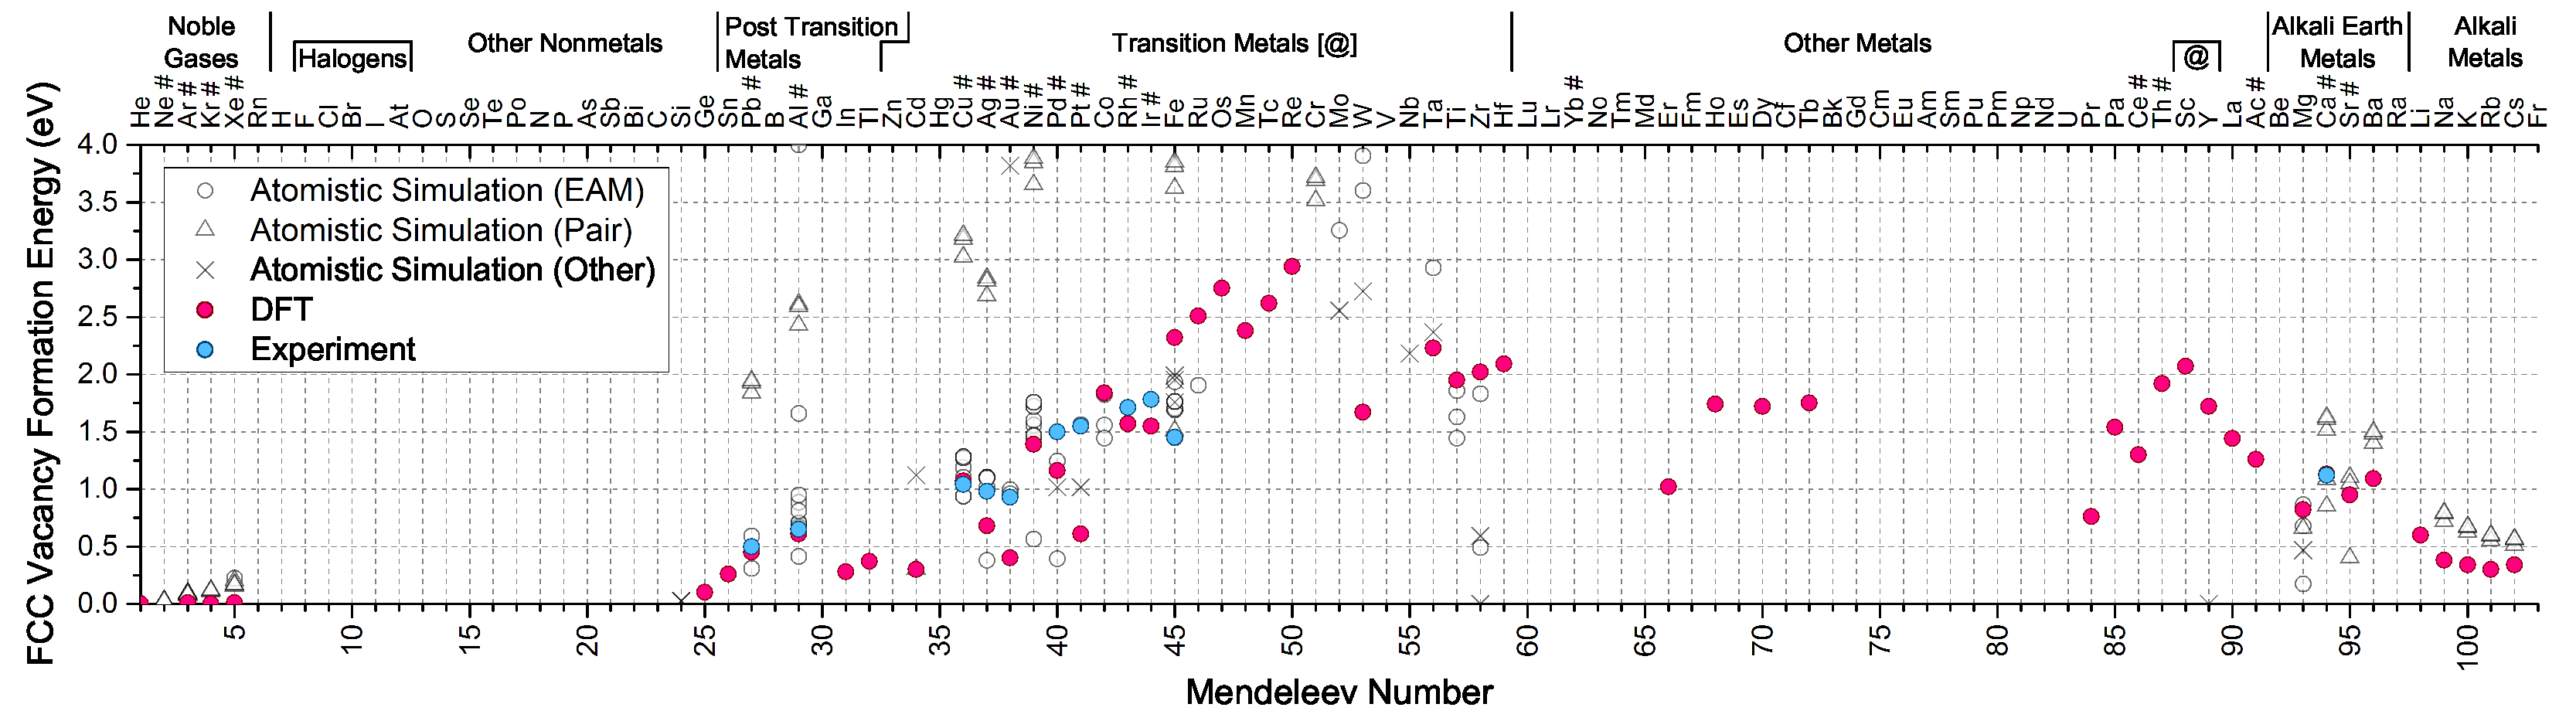
\includegraphics[trim=0 0 0 0,clip,width=1.0\textwidth]{fcc_vfe_new}}
\newline
\subfloat[][]{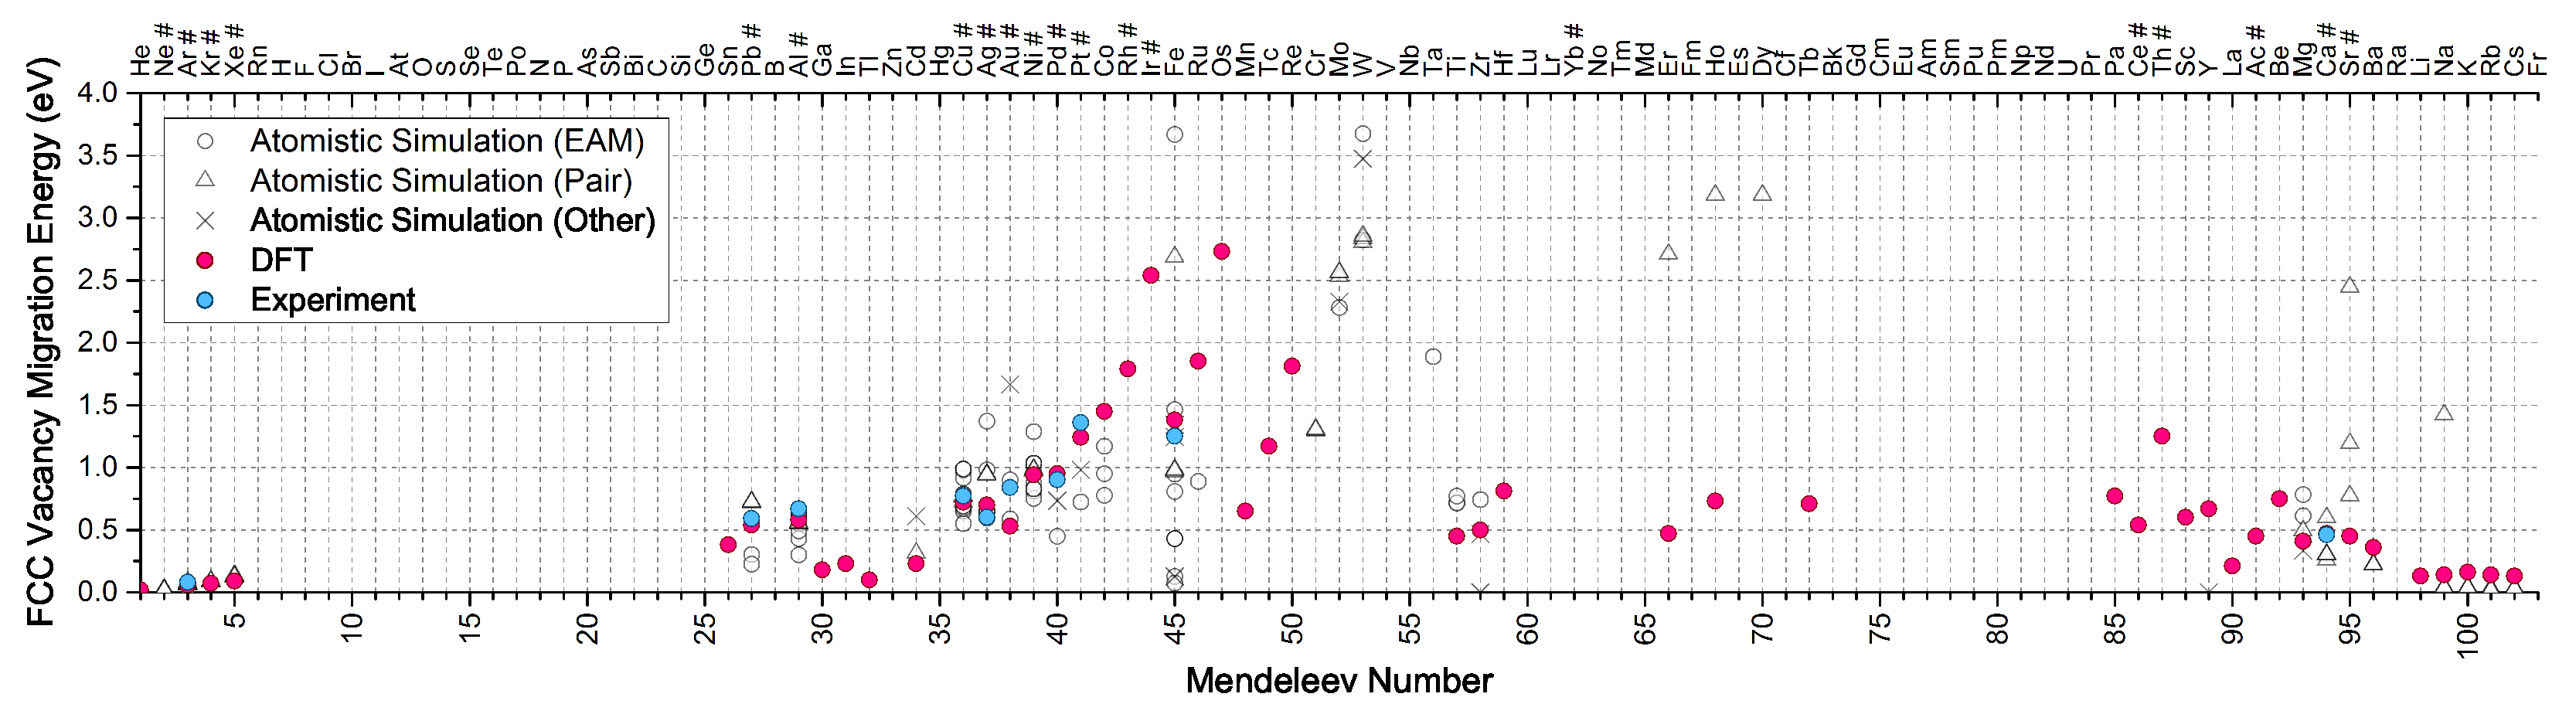
\includegraphics[trim=0 0 0 0,clip,width=1.0\textwidth]{fcc_vme_new}}
\newline
\subfloat[][]{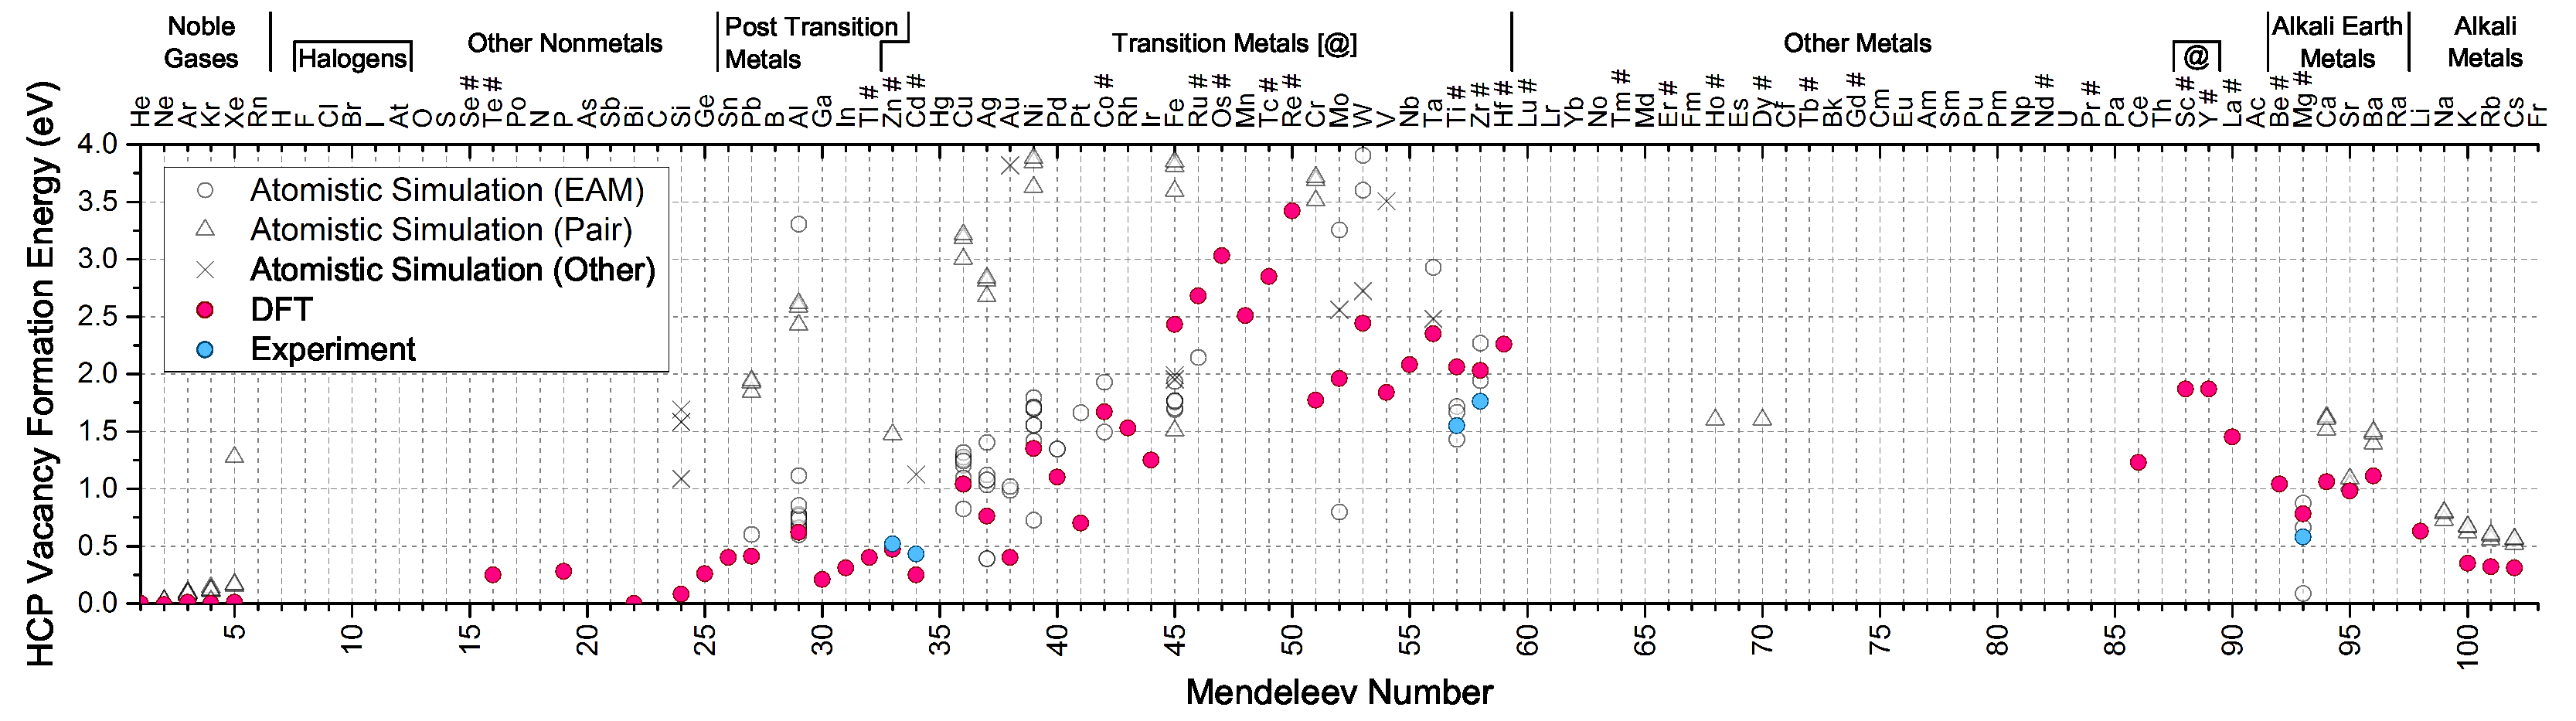
\includegraphics[trim=0 0 0 0,clip,width=1.0\textwidth]{hcp_vfe_new}}
\newline
\subfloat[][]{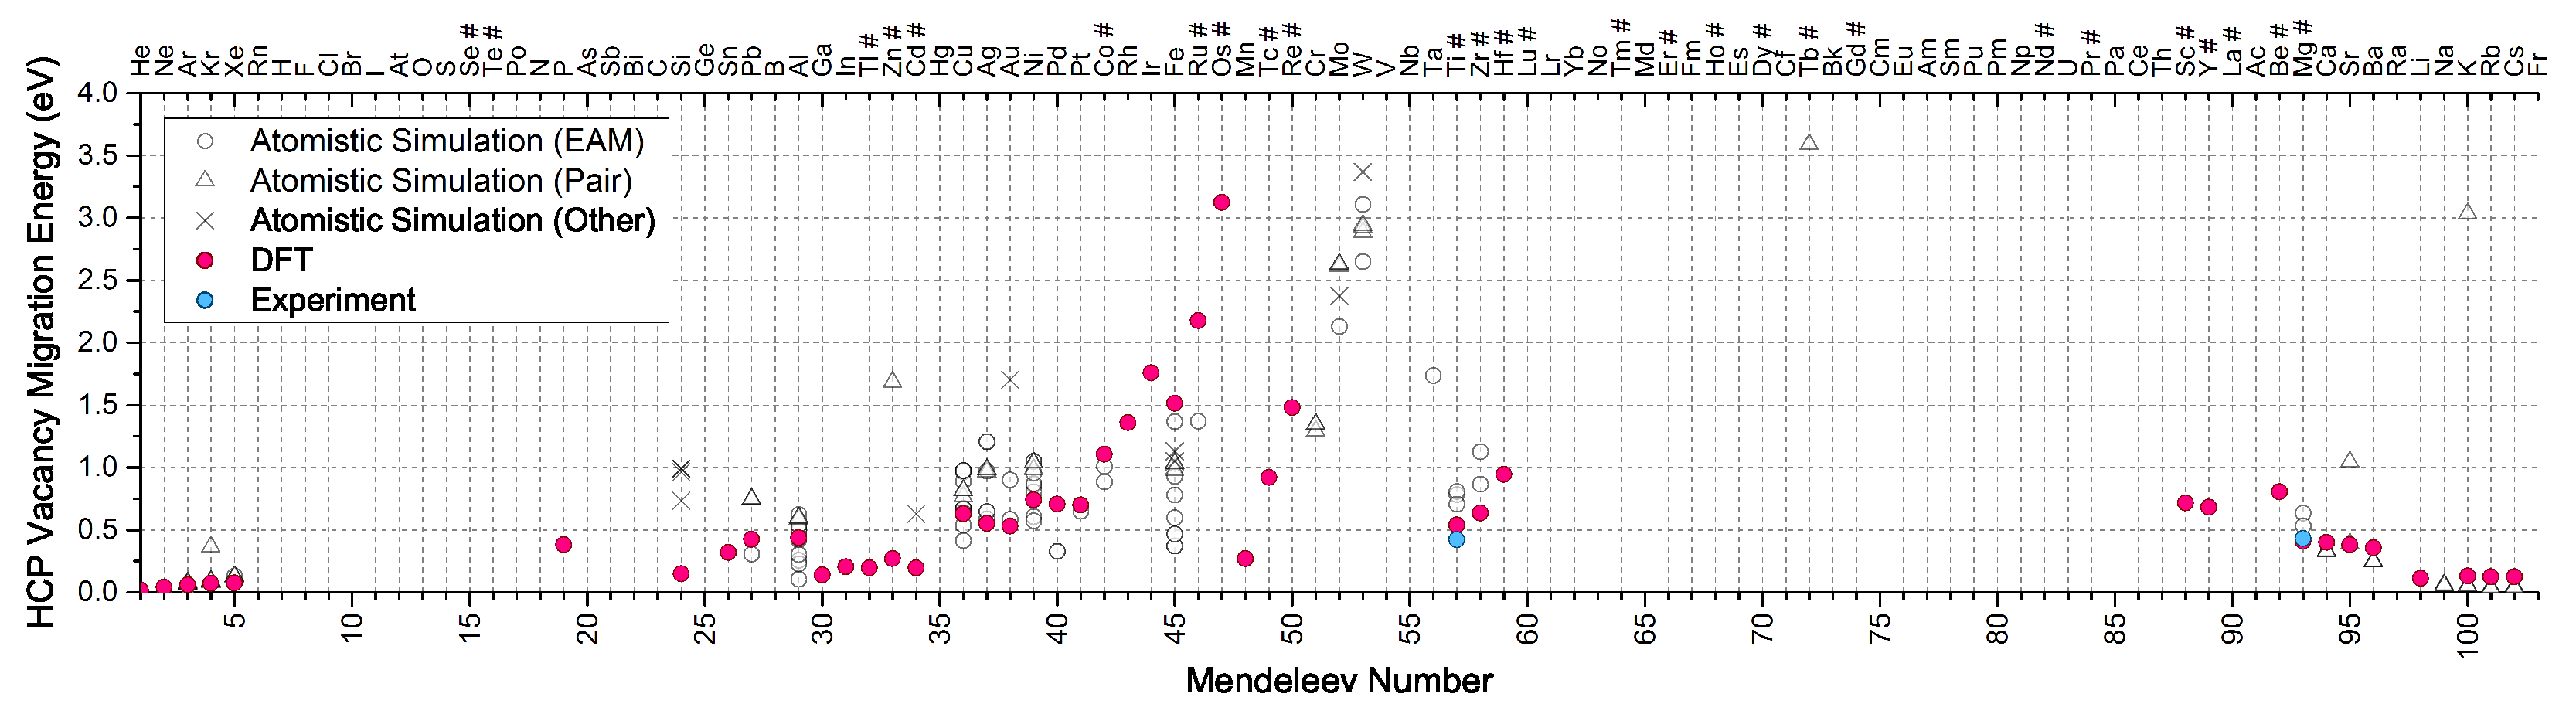
\includegraphics[trim=0 0 0 0,clip,width=1.0\textwidth]{hcp_vme_new}}
\caption{\label{fig:compare}
 Comparison of the results from our atomistic simulations and the reference data, where Fig.~(a) and (b) are the results for fcc structures, and Fig.~(c) and (d) are the results for hcp structures.
 The `\#' sign next to the symbol of each element indicates whether the structure presented by the figure is the element's natural state.
}
\end{figure*}

We can see from these figures that the EAM models, in general, produce similar VFE and VME as DFT calculations and experiments.
While most pairwise models tend to produce larger values for VFE, especially for elements with Mendeleev numbers ranging from 25 to 45, which correspond to the transition metals and the post-transition metals.

One explanation for the pairwise models to get larger VFE could be that pairwise models assume the strength of the bonds only depend on the distance between the two atoms.
They ignore the fact that the change in the number of bonds can also affect the strength of the bonds, and thus the energy.

To see this in detail, we exam the unrelaxed vacancy formation energy, $\mathit{UnrelaxedVFE}$, which the vacancy formation energy without position relaxation.
It consists of three parts, which can be expressed by
\begin{equation}
\label{eq:vfedecomp}
\mathit{UnrelaxedVFE} = N\cdot E_{bond} + \sum\Delta E_{bond} - E_{coh}
\end{equation}
where $N$ is the number of bonds surrounding each atom.
The first term corresponds to the breaking of the bonds between the vacant site and its nearest neighbors.
We ignore the contribution from breaking the bonds between the vacant site and its second nearest neighbors because it is much smaller than the first term.
The second term corresponds to the energy change in the remaining bonds.
And the third term is the cohesive energy, corresponding to the $n-1$ in Eq.~(\ref{eq:vfecalc}), which also equals to $N\cdot E_{bond}/2$, as the energy of each bond is shared between the two atoms it connects.
For all the pairwise models, we shall have $\mathit{UnrelaxedVFE}\approx E_{coh}$, as $\sum\Delta E_{bond}$ is zero; while for all the models that do take changes in the surrounding environment into consideration besides the distance between two atoms, we shall have $\mathit{UnrelaxedVFE}$ significantly different from $E_{coh}$.
In Table~\ref{tab:cohvfe} we show our verification: the pairwise models do get similar values for $\mathit{UnrelaxedVFE}$ and $E_{coh}$, while other types of models get significantly different values.
\begin{table}[!b]
\caption{\label{tab:cohvfe}
 Relationship between the cohesive energy, $E_{coh}$, and the unrelaxed vacancy formation energy, $\mathit{UnrelaxedVFE}$, calculated for fcc structures with different types of models.
 We can see that the pairwise models do get similar values for these two items while other types of models do get significantly different values.
 All the models can be found in the OpenKIM repository by the ID numbers shown in the footnotes.
}
\begin{ruledtabular}
\begin{tabular}{l c c}
 Model & $E_{coh}/\electronvolt$ & $\mathit{UnrelaxedVFE}/\electronvolt$\\
\hline
Pairwise Al\footnotemark[1] & 2.7004 & 2.7004\\
Pairwise Cu\footnotemark[1] & 3.2741 & 3.2741\\
EAM Al\footnotemark[2] & 3.3599 & 0.7691\\
EAM Cu\footnotemark[3] & 3.5193 & 1.2196\\
EMT Al\footnotemark[4] & 3.2788 & 0.9806\\
EMT Cu\footnotemark[4] & 3.2213 & 1.2788\\
\end{tabular}
\end{ruledtabular}
\footnotetext[1]{(ID: 411898953661\_001(Al) and 673777079812\_001(Cu)) Morse pair potential with parameters from Girifalco and Weizer, 1959.}
\footnotetext[2]{(ID: 651801486679\_001) EAM Al potential with parameters from Mishin et al., 1999.}
\footnotetext[3]{(ID: 179025990738\_001) EAM Cu potential with parameters from Ackland et al., 1987.}
\footnotetext[4]{(ID: 118428466217\_002) EMT implementation in ASAP by Jacobsen et al.}
\end{table}

===(Draft of draft below this line)===

In Table~\ref{tab:cohvfe}, we show an example of fcc copper: as we move the atom next to the vacant slight away from the original position, the change in the cohesive energy according to the EAM potential is about 40\% smaller than the value according to the pairwise potential.
This implies that as we create vacancy and remove bonds, the strength of the remaining bonds may decrease.
We propose that the vacancy formation energy can be expressed as
\begin{equation}
\label{eq:vfedecomp}
\mathit{VFE} = E_{cohesive} + \Delta E_{bonds, all} + \Delta E_{relaxation}
\end{equation}
Where $\Delta E_{bonds, all}$ is the change in the bond energy and the $\Delta E_{relaxation}$ is the change in energy due to position relaxation.
When we remove an atom, all the bonds associated with that atom are also removed, which means the energy change is $n \times E_{bond}$, where $n$ is the number of bonds surround each atom and $E_{bond}$ is the energy of a single bond.
Since each bond is associated with two atoms, thus the cohesive energy, $E_{cohesive}$, of an atom shall be the energy of half of the bonds associated with the atom, that is $n \times E_{bond}/2$.
Compare with Eq.~(\ref{eq:vfecalc}), we can get the first $E_{cohesive}$ term in Eq.~\ref{eq:vfedecomp}.
For pairwise potentials, $\Delta E_{bonds, all}$ is zero and $\Delta E_{relaxation}$ is usually much smaller than $E_{cohesive}$, so the vacancy formation energy according to them will be very close to the cohesive energy.
This can be verified with our data.
For example, with a pairwise potential for fcc copper, we will get the cohesive energy is 3.27 eV and the vacancy formation energy is 3.02 eV. We have also verified that without relaxation (no $\Delta E_{relaxation}$), the unrelaxed vacancy formation energy is also 3.27 eV, same as $E_{cohesive}$.

\begin{table}
\caption{\label{tab:cu}
 Change in the cohesive energy of fcc copper as we move the atom next to the vacant slight slightly along the $x$ direction away from the original position.
}
\begin{ruledtabular}
\begin{tabular}{c c c}
 Displacement (\AA) & EAM\footnotemark[1] (eV) & Pairwise\footnotemark[2] (eV)\\
\hline
0.01 & 0.000 & 0.000 \\
0.02 & 0.001 & 0.002 \\
0.04 & 0.005 & 0.009 \\
0.08 & 0.021 & 0.037 \\
0.16 & 0.092 & 0.148 \\
0.32 & 0.407 & 0.596 \\
0.64 & 1.649 & 2.440 \\
1.28 & 5.383 & 9.306 \\
2.56 & 13.37 & 41.91 \\
5.12 & 10.31 & 22.04 \\
\end{tabular}
\end{ruledtabular}
\footnotetext[1]{EAM\_Dynamo\_Ackland\_Tichy\_Cu.}
\footnotetext[2]{Pair\_Morse\_Shifted\_GirifalcoWeizer\_LowCutoff\_Cu.}
\end{table}

For pairwise potentials, the bond energy per atom increase linearly with the number of bonds.
However, experiments show there is a quadratic relationship between them.
This implies that when we remove a bond, the strength of the remaining bonds will be weakened.
Therefore, the change in energy during position relaxation will be smaller than if the bond strength remains the same.
And this change in energy is exactly the main component of the vacancy formation energy.

Other types of potentials sometimes also produce accurate results but are only available to a few elements.
This suggests that right now in general EAM is the most promising method for describing vacancy effects.
We believe there are several reasons why EAM outperforms other methods:
\begin{enumerate}
\item EAM incorporates the multibody effects, which is crucial for describing the interaction between atoms.
\item The training data for the EAM potentials usually includes both experimental data and DFT calculation results.
\item For the EAM potentials, most of the information contained in the training data is kept into the potential models, while for other fixed-form potentials, lots of information is lost during the fitting process.
\end{enumerate}

In Table~\ref{tab:bestmodels}, we list the models currently available on OpenKIM that are most consistent with DFT and experiments.
They are selected based on the mean absolute percentage error (MAPE), a measure of prediction accuracy of models used in statistics, which in this case is defined as the average relative error to our reference data
\begin{equation}
\label{eq:mape}
\mathit{MAPE} = \frac{1}{n}\sum_i\left|\frac{C_i-R_i}{R_i}\right|
\end{equation}
Here $n$ is the number of reference data available for the items we successfully calculate, $C_i$ is the calculated value, and $R_i$ is the reference value.
The value of $\mathit{MAPE}$ for each model in this table is shown in column 4.
Note that in our reference data, the mean absolute percentage error between the DFT results and experimental results is 27.87\%.
Comparing to this, we can see that for most of the elements in this table, there exists a potential that can produce reasonably accurate results.
These potentials are all good candidates for atomistic simulation when vacancy effects are significant.

We can also see from these two tables that for nearly all the elements that have EAM potentials, the EAM potentials are selected as the best models in Table~\ref{tab:bestmodels} according to the criteria above.
Only in very few cases, other types of potentials perform better than the EAM potentials.
This is consistent with our previous analysis.

\subsection{\label{sec:calcvsprop}Relationship to Other Properties}

\begin{figure*}
\centering
\noindent\ignorespaces
\subfloat[][]{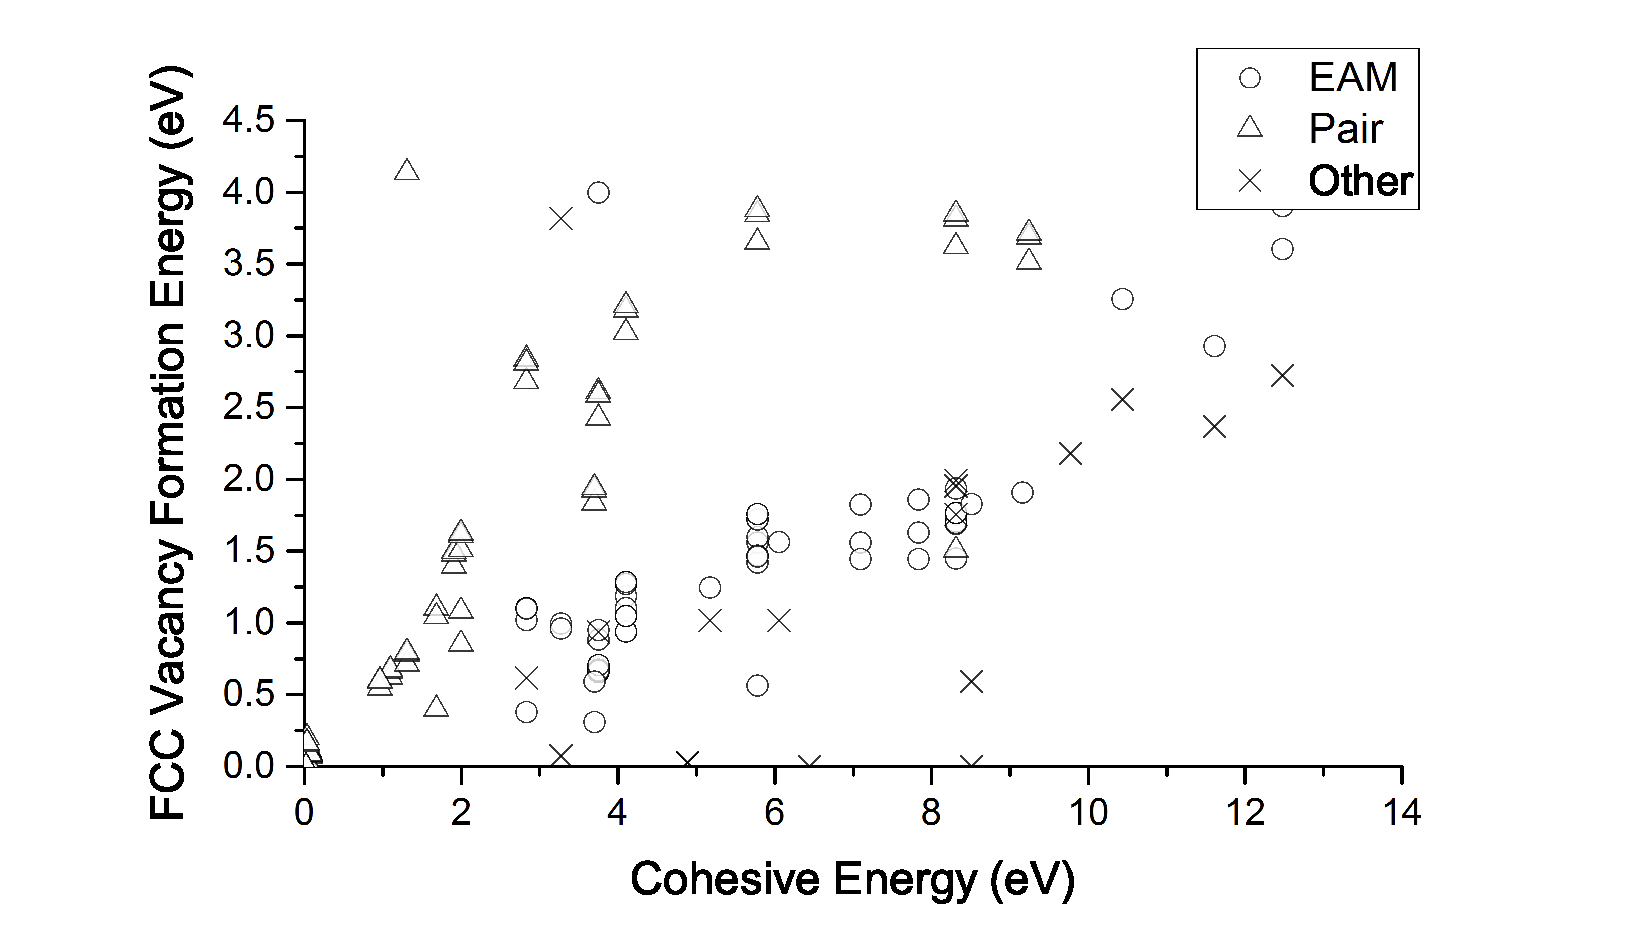
\includegraphics[trim=0 0 0 0,clip,width=0.48\textwidth]{vfe_energy_fcc}}\hfill
\subfloat[][]{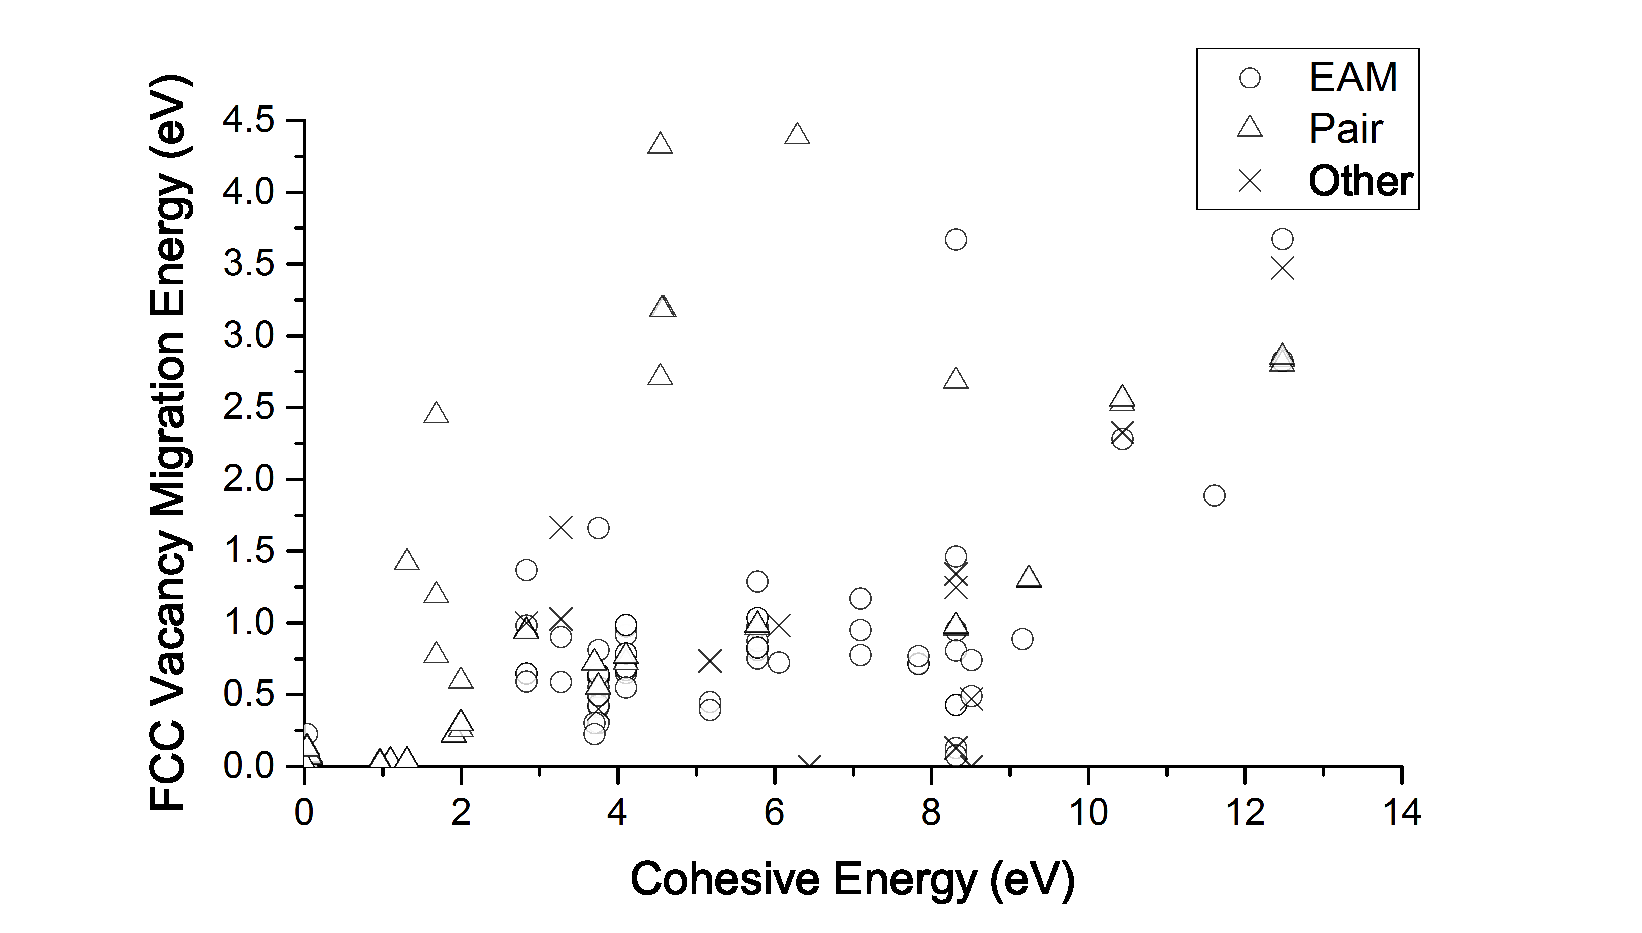
\includegraphics[trim=0 0 0 0,clip,width=0.48\textwidth]{vme_energy_fcc}}
\newline
\noindent\ignorespaces
\subfloat[][]{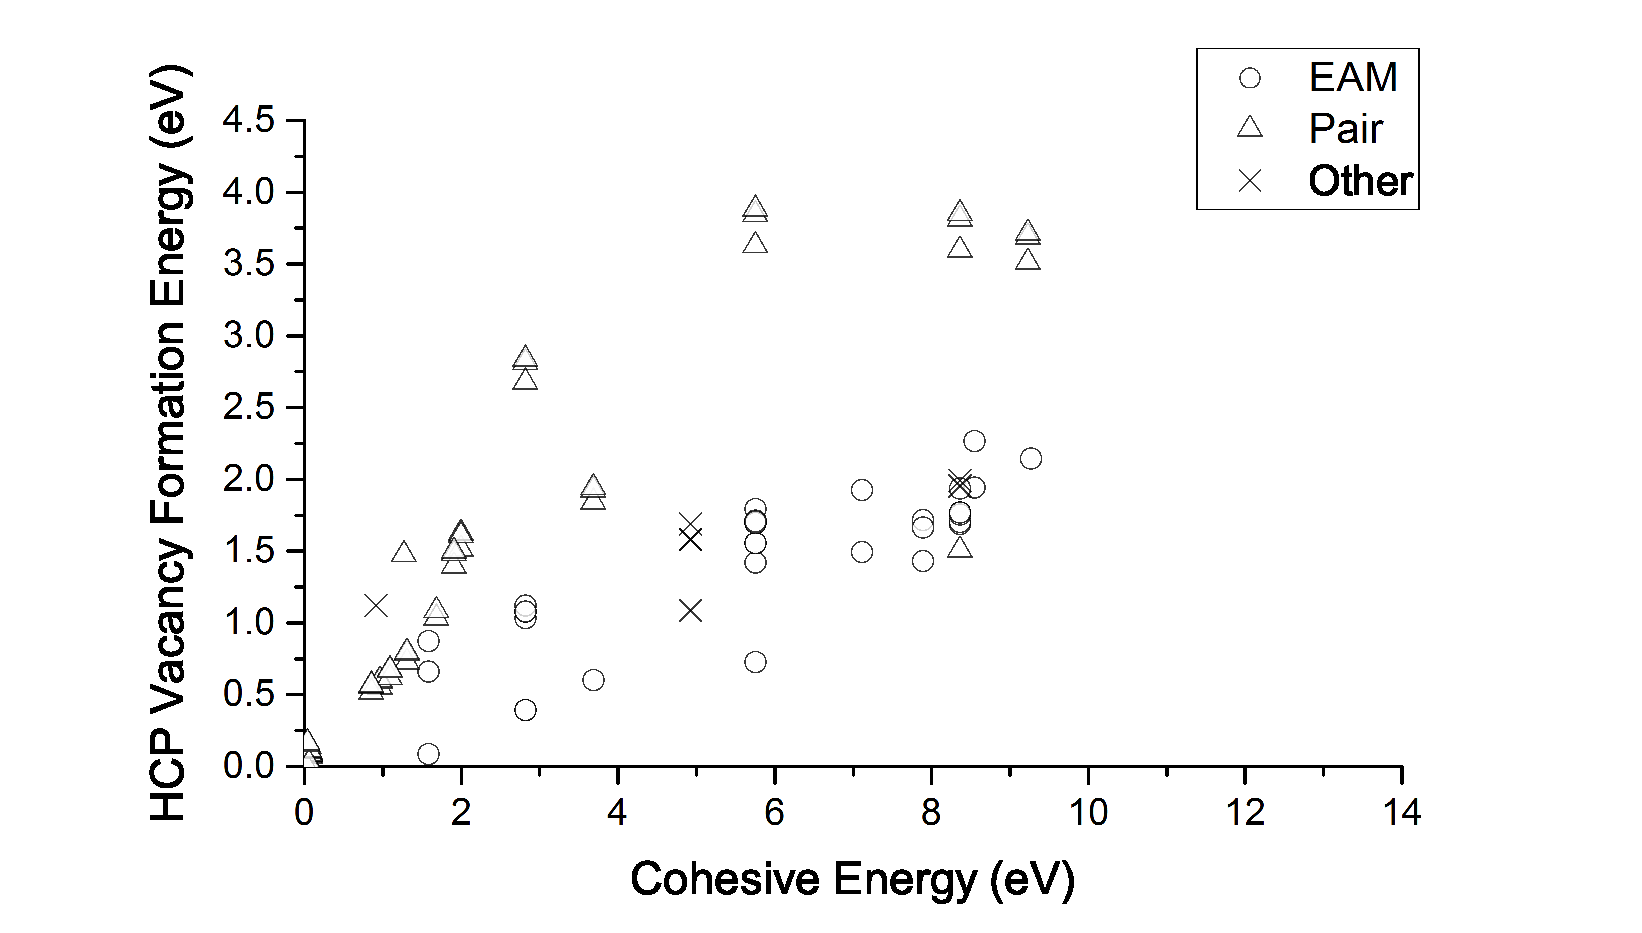
\includegraphics[trim=0 0 0 0,clip,width=0.48\textwidth]{vfe_energy_hcp}}\hfill
\subfloat[][]{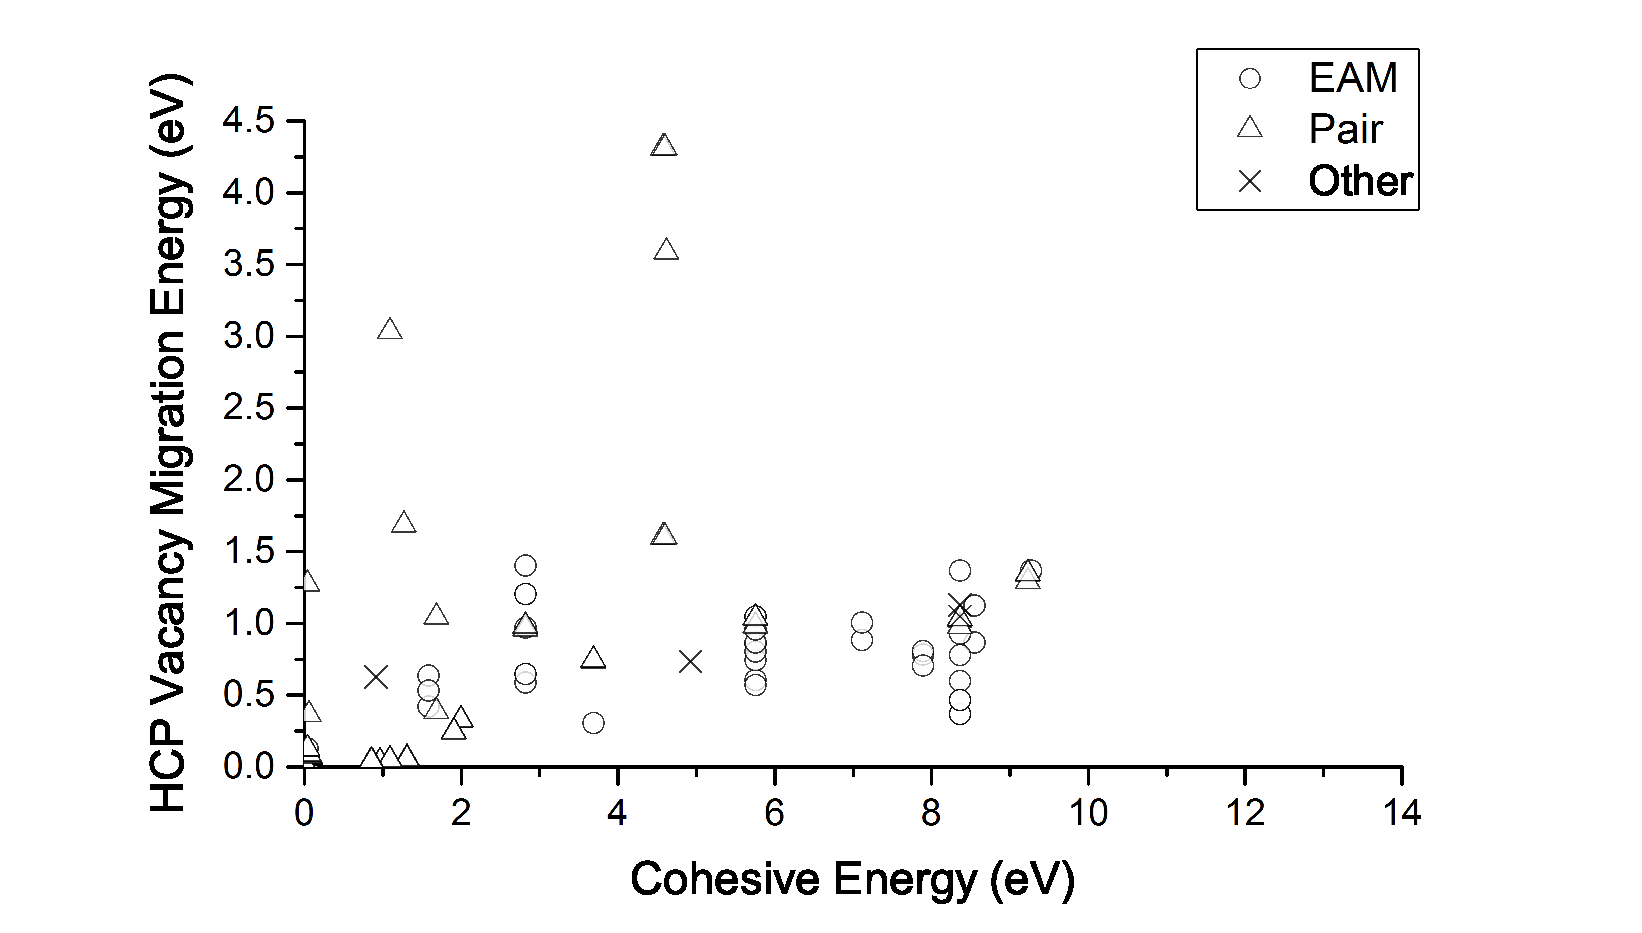
\includegraphics[trim=0 0 0 0,clip,width=0.48\textwidth]{vme_energy_hcp}}
\newline
\noindent\ignorespaces
\subfloat[][]{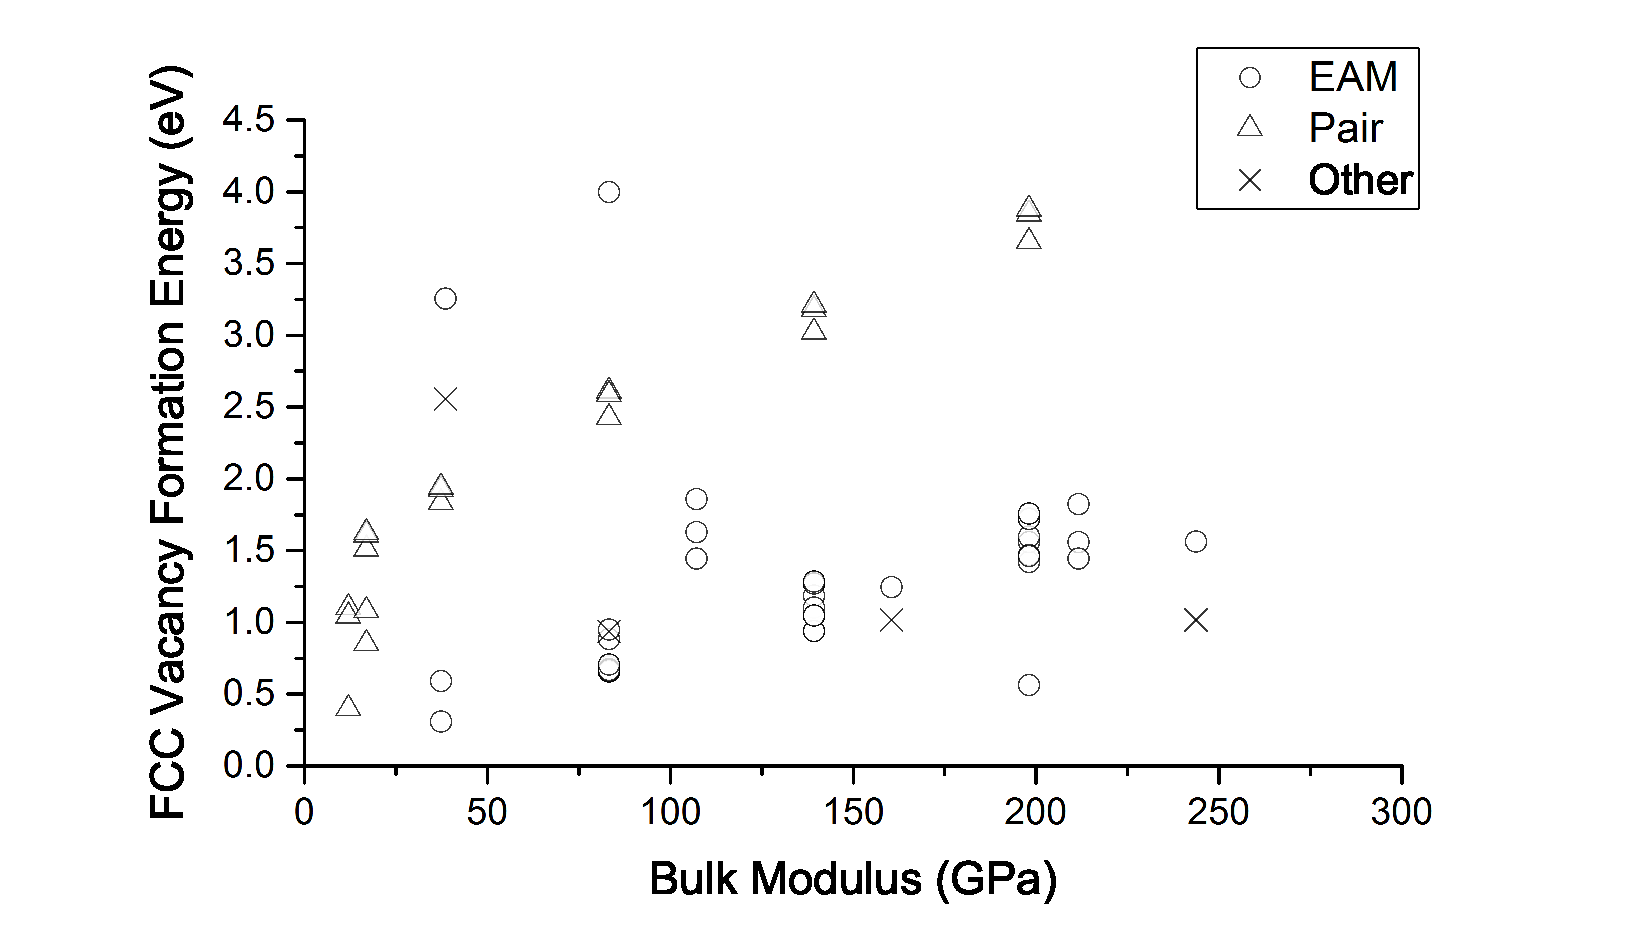
\includegraphics[trim=0 0 0 0,clip,width=0.48\textwidth]{vfe_bulk_fcc}}\hfill
\subfloat[][]{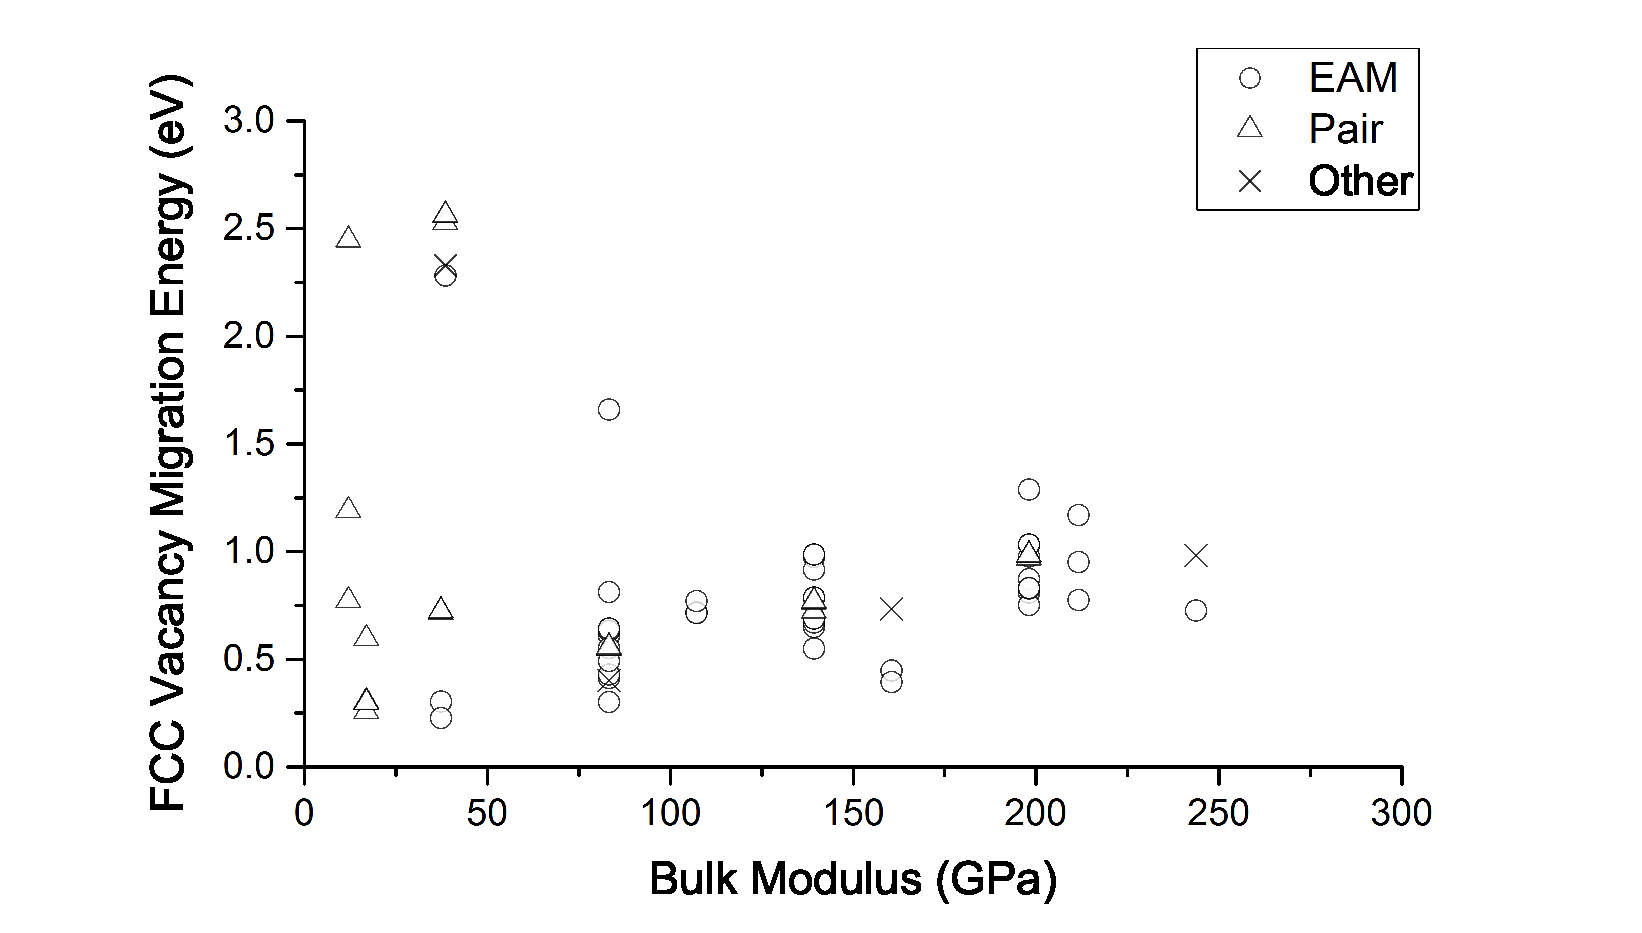
\includegraphics[trim=0 0 0 0,clip,width=0.48\textwidth]{vme_bulk_fcc}}
\newline
\noindent\ignorespaces
\subfloat[][]{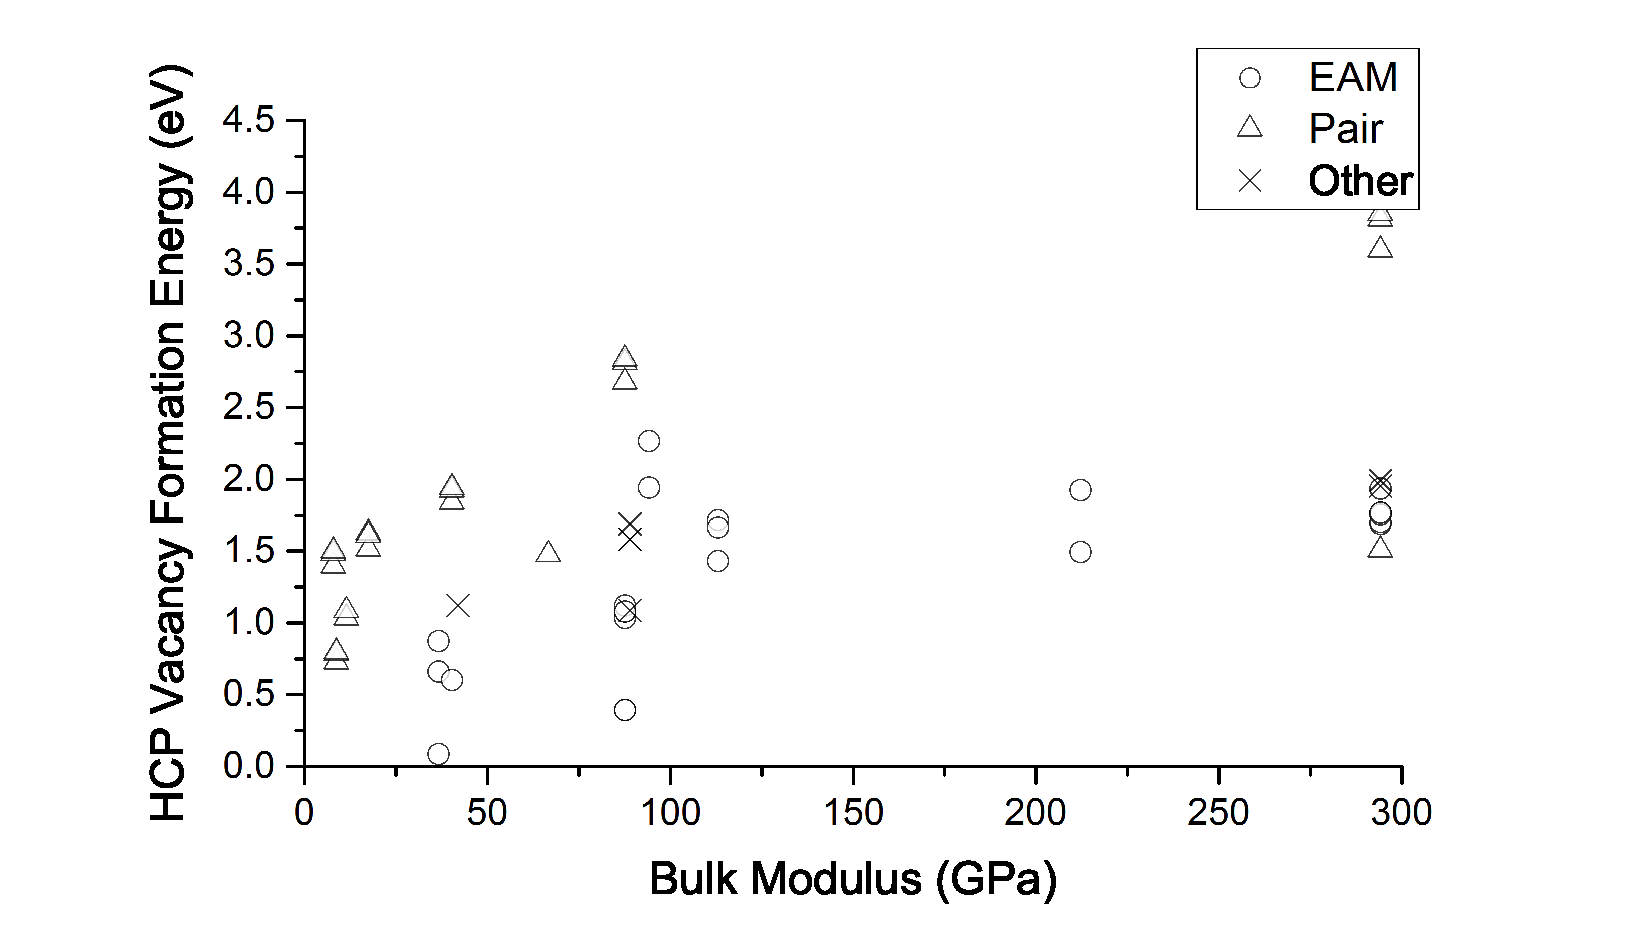
\includegraphics[trim=0 0 0 0,clip,width=0.48\textwidth]{vfe_bulk_hcp}}\hfill
\subfloat[][]{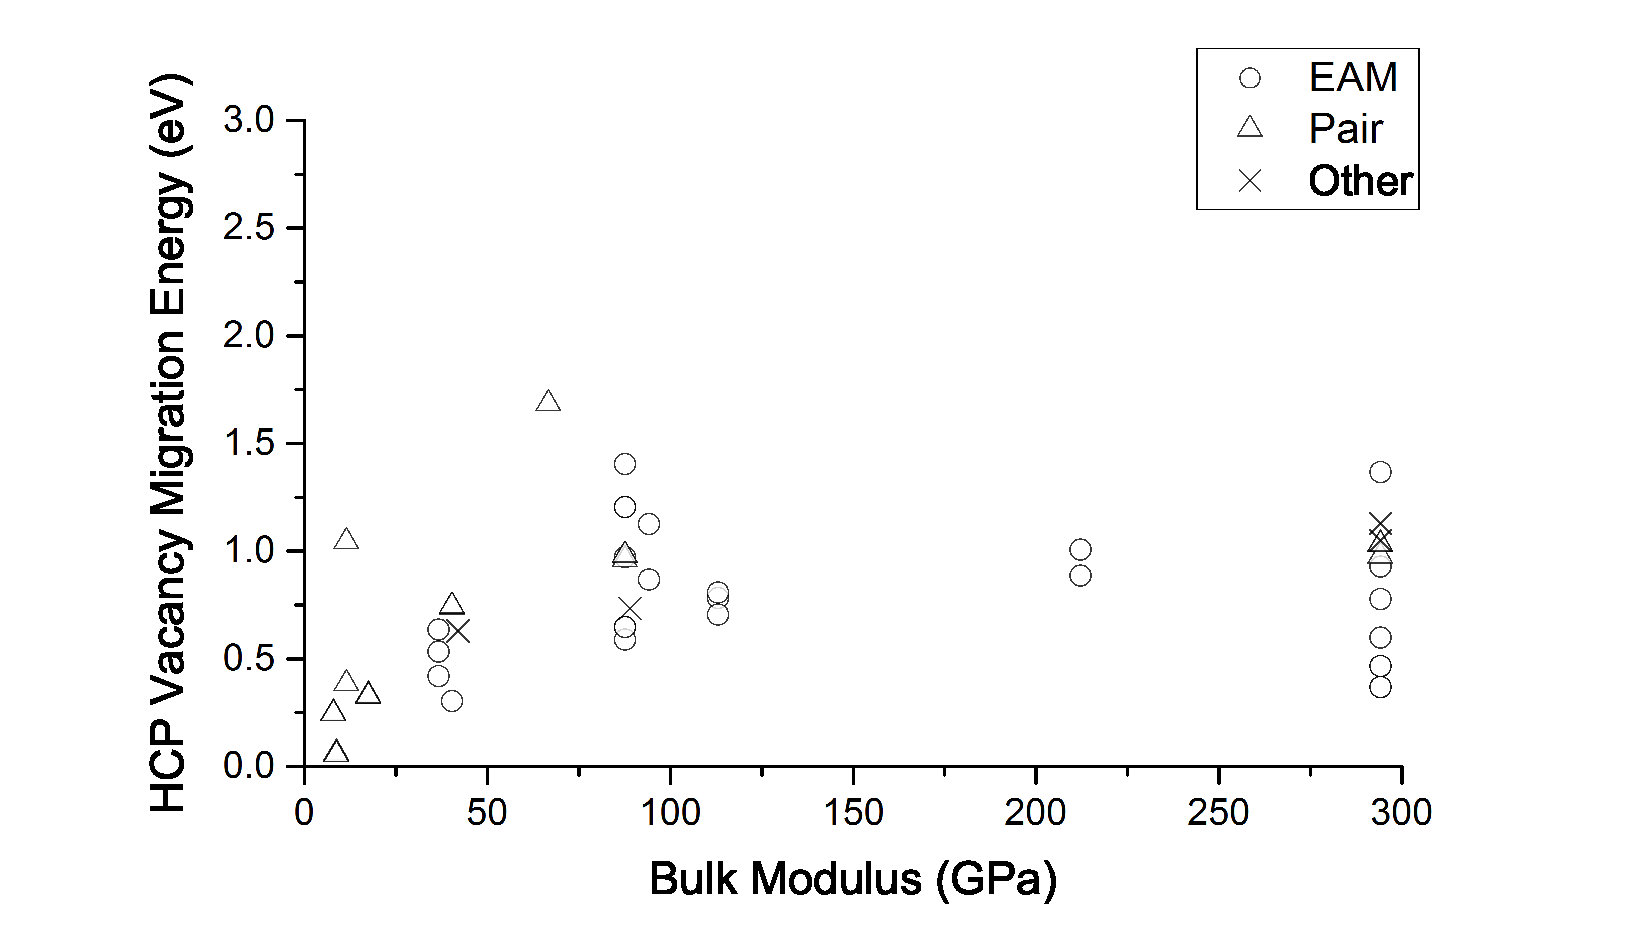
\includegraphics[trim=0 0 0 0,clip,width=0.48\textwidth]{vme_bulk_hcp}}
\caption{\label{fig:vsenergy}
 VFE and VME versus cohesive energy and bulk modulus.
}
\end{figure*}

We plot the vacancy property results from our atomistic simulation against cohesive energy and bulk modulus in Fig.~\ref{fig:vsenergy}.
Both the cohesive energy and bulk modulus are obtained from the Materials Project \cite{jain2013commentary,de2015charting}.
Here we use the same symbol as in Fig.~\ref{fig:compare}: the circles represent embedded-atom method (EAM), the triangles represent pairwise potentials, and the cross signs represent all the other types of potentials, such as three-body potentials.

We can see from these plots that as cohesive energy increases, vacancy formation energy and migration energy also increase.
This is consistent with previous results from DFT \cite{angsten2014elemental}.

\section{\label{sec:conclusion}Conclusion}

In this study, we assess the quality of interatomic models currently available in the OpenKIM repository \url{https://openkim.org/intro-models/}, in terms of their ability to describing vacancy-related properties.

We first develop tests using the OpenKIM API to perform the atomistic calculation of three most important monovacancy properties, the vacancy formation energy, the vacancy migration energy and the relaxation energy, for all the available interatomic models.
Then we compare the calculation results with reference data from density functional (DFT) calculations and experiments by plotting them on the same graphs.
These figures show that the EAM potentials, in general, agree with DFT calculations and experiments, while the pairwise potentials tend to overestimate the vacancy formation energy.
We offer an explanation for this: the pairwise potentials neglect the fact that as we remove an atom and create a vacant site, we decrease the number of bonds, which will, in turn, decrease the strength of the remaining bonds and thus the energy change during the relaxation.
By using mean absolute percentage error as a measure of the deviation from the reference data to our results, we identify the most promising interatomic models for defect-related simulations for each element.
The types of these models agree with our previous analysis: for elements that have EAM potentials, one of the EAM potentials is usually selected as the best model according to the criteria above.

We also plot the results against other elemental properties.
The plots show that vacancy formation energy and vacancy migration energy increase with cohesive energy and bulk modulus, which is consistent with previous DFT based studies \cite{angsten2014elemental}.

\section{\label{sec:conclusion}Future Works}

First of all, more accurate reference data will be extremely beneficial for improving the accuracy of our assessment.
This may be done by improvements in the algorithm used in DFT calculations or the procedure used in experiments.
The usage of other computational methods, such as quantum chemistry methods or quantum Monte Carlo may also help.

In addition, the way we select the best models also worth further exploration.
The measure used in this study is the mean absolute percentage error, which is widely used but has some biases \cite{mayer1993statistical}.
It is possible that through some statistical analysis we can get a more suitable measure for this specific situation, and select the best model to perform the calculation we need accordingly, or select multiple models to perform the same calculation and assigning different weight to the result produced by each model accordingly and calculate the weighted average as the final result \cite{frederiksen2004bayesian}.

Finally, for models with tunable parameters, it would be beneficial to have a unified system that can give the best parameter set (or sets) based on the reference data and the requirement of the user.

%\begin{acknowledgments}
%We wish to acknowledge the support of the author community in using
%REV\TeX{}, offering suggestions and encouragement, testing new versions,
%\dots.
%\end{acknowledgments}

\appendix

\section{\label{app:data}Scripts for Retrieving Data From OpenKIM}

In this section, we list the scripts for retrieving the data used in this paper from OpenKIM.

\section{\label{app:results}Listing of Results}
All the results in this work are listed in Table~\ref{tab:fccresults} for archive.
The most updated data can be found at the OpenKIM website \url{https://openkim.org/}.

The calculations are performed with the algorithm described in Section~\ref{sec:method}.
The code that implements this algorithm can also be found on the OpenKIM website.
Note that for some model-structure pairs, the calculation can't terminate within the time allowed, or produce results that are far from reality.
These items are marked as ``-'' in the two tables mentioned above.

\setlength\LTleft{0pt}
\setlength\LTright{0pt}
\setlength{\LTcapwidth}{7in}

\begin{longtable*}{@{\extracolsep{\fill}} c l c c c c c c}
 \caption{\label{tab:fccresults}
  Vacancy formation energy (VFE), migration energy (VME) and relaxation volume (VRV) calculated from atomistic simulations.
  See Section~\ref{sec:method} for the algorithm used in obtaining these results.
 }\\% \noalign{\nobreak\vspace{1pt}}%
 \toprule
 \multirow{2}{*}{Symbol} & \multirow{2}{*}{Model} & \multicolumn{2}{c}{VFE (eV)} & \multicolumn{2}{c}{VME (eV)} & \multicolumn{2}{c}{VRV ($\AA^3$)}\\
  & & fcc & hcp & fcc & hcp & fcc & hcp\\
 \colrule
 \nobreak\vspace{0.5pt}%
 \endfirsthead
 \caption{
  (continued)
 }\\
 \toprule
 \multirow{2}{*}{Symbol} & \multirow{2}{*}{Model} & \multicolumn{2}{c}{VFE (eV)} & \multicolumn{2}{c}{VME (eV)} & \multicolumn{2}{c}{VRV ($\AA^3$)}\\
  & & fcc & hcp & fcc & hcp & fcc & hcp\\ \colrule
 \endhead
 \botrule
 \endfoot
 \botrule
 \endlastfoot
 Ag & EAM\_Dynamo\_Ackland\_Tichy\_Ag & 1.02 & 1.03 & 0.98 & 0.97 & - & - \\
 Ag & EAM\_Dynamo\_Hale\_Wong\_pairHybrid\_PdAgH & 0.38 & 0.39 & 1.37 & 1.21 & - & - \\
 Ag & EAM\_Dynamo\_Hale\_Wong\_pairMorse\_PdAgH & - & 0.39 & - & 1.21 & - & - \\
 Ag & EAM\_Dynamo\_Williams\_Mishin\_Ag & 1.10 & 1.08 & 0.65 & 0.65 & - & - \\
 Ag & EAM\_Dynamo\_Williams\_Mishin\_CuAg & 1.10 & 1.08 & 0.65 & 0.65 & - & - \\
 Ag & EAM\_Dynamo\_Wu\_Trinkle\_CuAg & 1.10 & - & 0.65 & 1.40 & - & - \\
 Ag & EAM\_Dynamo\_Zhou\_Johnson\_Ag & 1.10 & 1.12 & 0.59 & 0.59 & - & - \\
 Ag & EMT\_Asap\_Standard\_Jacobsen\_Stoltze\_Norskov\_AlAgAuCuNiPdPt & 0.62 & - & 1.00 & - & - & - \\
 Ag & Pair\_Morse\_Shifted\_GirifalcoWeizer\_HighCutoff\_Ag & 2.84 & 2.84 & 0.95 & 0.98 & 2.20 & 2.13 \\
 Ag & Pair\_Morse\_Shifted\_GirifalcoWeizer\_LowCutoff\_Ag & 2.68 & 2.68 & 0.94 & 0.96 & 1.98 & 1.95 \\
 Ag & Pair\_Morse\_Shifted\_GirifalcoWeizer\_MedCutoff\_Ag & 2.81 & 2.81 & 0.94 & 0.98 & 1.79 & 1.97 \\
 Al & EAM\_Dynamo\_Angelo\_Moody\_NiAlH & - & 0.60 & - & 0.10 & - & - \\
 Al & EAM\_Dynamo\_Cai\_Ye\_AlCu & - & - & 0.81 & 0.85 & - & - \\
 Al & EAM\_Dynamo\_Ercolessi\_Adams\_Al & 0.69 & 0.78 & 0.61 & 0.44 & - & - \\
 Al & EAM\_Dynamo\_Mendelev\_Asta\_AlMg & 0.66 & 0.64 & 0.64 & 0.54 & - & - \\
 Al & EAM\_Dynamo\_Mendelev\_Kramer\_Al & 0.66 & 0.64 & 0.64 & 0.54 & - & - \\
 Al & EAM\_Dynamo\_Mendelev\_Srolovitz\_AlFe & - & 0.66 & 0.41 & 0.62 & - & - \\
 Al & EAM\_Dynamo\_Mishin\_Farkas\_Al & 0.68 & 0.74 & 0.63 & 0.44 & - & - \\
 Al & EAM\_Dynamo\_Mishin\_Mehl\_NiAl & 4.00 & 3.31 & - & - & - & - \\
 Al & EAM\_Dynamo\_Mishin\_NiAl & 0.71 & - & 0.64 & - & - & - \\
 Al & EAM\_Dynamo\_PurjaPun\_Mishin\_NiAl & 0.68 & - & 0.63 & 1.12 & - & - \\
 Al & EAM\_Dynamo\_Sturgeon\_Laird\_Al & 0.89 & - & 0.55 & - & - & - \\
 Al & EAM\_Dynamo\_Vailhe\_Farkas\_CoAl & - & 0.68 & 1.66 & 0.23 & - & - \\
 Al & EAM\_Dynamo\_Winey\_Kubota\_Al & 0.66 & 0.64 & 0.43 & 0.30 & - & - \\
 Al & EAM\_Dynamo\_Zhou\_Johnson\_Al & 0.67 & 0.71 & 0.30 & 0.26 & - & - \\
 Al & EAM\_Dynamo\_Zope\_Mishin\_Al & 0.71 & 0.76 & 0.64 & 0.49 & - & - \\
 Al & EAM\_Dynamo\_Zope\_Mishin\_TiAl & 0.95 & 0.76 & 0.49 & 0.49 & - & - \\
 Al & EMT\_Asap\_Standard\_Jacobsen\_Stoltze\_Norskov\_AlAgAuCuNiPdPt & 0.94 & - & 0.40 & - & - & - \\
 Al & Pair\_Morse\_Shifted\_GirifalcoWeizer\_HighCutoff\_Al & 2.61 & 2.62 & 0.55 & 0.60 & 8.62 & 3.15 \\
 Al & Pair\_Morse\_Shifted\_GirifalcoWeizer\_LowCutoff\_Al & 2.43 & 2.43 & 0.55 & 0.58 & 3.18 & 2.57 \\
 Al & Pair\_Morse\_Shifted\_GirifalcoWeizer\_MedCutoff\_Al & 2.59 & 2.59 & 0.56 & 0.59 & 3.35 & 3.14 \\
 Ar & Pair\_LJ\_Smooth\_Bernardes\_Ar & 0.07 & 0.07 & 0.06 & 0.06 & 0.77 & 0.89 \\
 Ar & Pair\_Lennard\_Jones\_Shifted\_Bernardes\_HighCutoff\_Ar & 0.09 & 0.09 & 0.07 & 0.07 & 1.36 & 1.37 \\
 Ar & Pair\_Morse\_Sigmoid\_Jelinek\_Ar & 0.00 & 0.00 & 0.00 & 0.00 & - & - \\
 Ar & Pair\_Morse\_Shifted\_Jelinek\_Ar & 0.09 & 0.09 & 0.07 & 0.07 & 0.87 & 0.88 \\
 Ar & Pair\_Morse\_Smoothed90\_Jelinek\_Ar & 0.09 & 0.09 & 0.07 & 0.07 & 0.86 & 0.88 \\
 Ar & Pair\_Lennard\_Jones\_Shifted\_Bernardes\_LowCutoff\_Ar & 0.08 & 0.08 & 0.06 & 0.06 & 0.93 & 1.06 \\
 Ar & Pair\_Lennard\_Jones\_Truncated\_Nguyen\_Ar & 0.09 & 0.09 & 0.08 & 0.07 & - & 24.83 \\
 Ar & Pair\_Lennard\_Jones\_Shifted\_Bernardes\_MedCutoff\_Ar & 0.09 & 0.09 & 0.07 & 0.07 & 1.34 & 1.33 \\
 Au & EMT\_Asap\_Standard\_Jacobsen\_Stoltze\_Norskov\_AlAgAuCuNiPdPt & 0.07 & - & 1.03 & - & - & - \\
 Au & EAM\_Dynamo\_Zhou\_Johnson\_Au & 1.00 & 1.02 & 0.59 & 0.59 & - & - \\
 Au & EAM\_Dynamo\_Ackland\_Tichy\_Au & 0.96 & 0.99 & 0.90 & 0.90 & - & - \\
 Au & MorseEIP\_GuthikondaElliott\_2011\_AuCd & 3.82 & 3.82 & 1.67 & 1.70 & 1.49 & 1.49 \\
 Ca & LennardJones612\_Universal & 0.85 & - & 0.26 & - & - & - \\
 Ca & Pair\_Morse\_Shifted\_GirifalcoWeizer\_LowCutoff\_Ca & 1.51 & 1.51 & 0.30 & 0.33 & 9.20 & 9.21 \\
 Ca & LennardJones612\_UniversalShifted & 1.08 & - & 0.60 & - & - & - \\
 Ca & Pair\_Morse\_Shifted\_GirifalcoWeizer\_MedCutoff\_Ca & 1.61 & 1.61 & 0.30 & 0.33 & 9.84 & 9.92 \\
 Ca & Pair\_Morse\_Shifted\_GirifalcoWeizer\_HighCutoff\_Ca & 1.63 & 1.63 & 0.30 & 0.33 & 10.07 & 10.07 \\
 Ba & Pair\_Morse\_Shifted\_GirifalcoWeizer\_LowCutoff\_Ba & 1.40 & 1.39 & 0.22 & 0.25 & 16.77 & 16.00 \\
 Ba & Pair\_Morse\_Shifted\_GirifalcoWeizer\_MedCutoff\_Ba & 1.48 & 1.48 & 0.22 & 0.25 & 17.75 & 17.48 \\
 Ba & Pair\_Morse\_Shifted\_GirifalcoWeizer\_HighCutoff\_Ba & 1.50 & 1.50 & 0.22 & 0.25 & 18.37 & 17.86 \\
 Co & EAM\_Dynamo\_Zhou\_Johnson\_Co & 1.83 & 1.93 & 0.78 & 0.89 & - & - \\
 Co & EAM\_Dynamo\_PurjaPun\_Mishin\_Co & 1.56 & 1.49 & 0.95 & 1.01 & - & - \\
 Co & EAM\_Dynamo\_Vailhe\_Farkas\_CoAl & 1.44 & - & 1.17 & 28.50 & - & - \\
 Cr & Pair\_Morse\_Shifted\_GirifalcoWeizer\_LowCutoff\_Cr & 3.51 & 3.51 & 1.29 & 1.29 & 1.31 & 2.15 \\
 Cr & Pair\_Morse\_Shifted\_GirifalcoWeizer\_MedCutoff\_Cr & 3.69 & 3.69 & 1.30 & 1.35 & 1.39 & 1.38 \\
 Cr & Pair\_Morse\_Shifted\_GirifalcoWeizer\_HighCutoff\_Cr & 3.72 & 3.72 & 1.30 & 1.35 & 1.42 & 1.40 \\
 Cu & EAM\_Dynamo\_Hoyt\_Garvin\_PbCu & 1.28 & 1.28 & 0.67 & 0.67 & - & - \\
 Cu & EAM\_Dynamo\_Cai\_Ye\_AlCu & 1.27 & 1.27 & 0.65 & 0.66 & - & - \\
 Cu & EAM\_Dynamo\_Foiles\_Baskes\_Universal3\_Cu & 1.28 & 1.28 & 0.67 & 0.67 & - & - \\
 Cu & EAM\_Dynamo\_Bonny\_Pasianot\_FeCuNi & 1.27 & 1.25 & 0.69 & 0.67 & - & - \\
 Cu & EAM\_Dynamo\_Ackland\_Tichy\_Cu & 1.19 & 1.20 & 0.98 & 0.97 & - & - \\
 Cu & EAM\_Dynamo\_Mendelev\_King\_Cu & 1.11 & 1.09 & 0.92 & 0.89 & - & - \\
 Cu & EAM\_Dynamo\_Onat\_Durukanoglu\_CuNi & 0.94 & 18.88 & 0.79 & - & - & - \\
 Cu & EAM\_Dynamo\_Mendelev\_Kramer\_Cu & 1.05 & 1.04 & 0.99 & 0.97 & - & - \\
 Cu & EAM\_Dynamo\_Mishin\_Mehl\_Cu & 1.27 & 1.25 & 0.69 & 0.67 & - & - \\
 Cu & EAM\_Dynamo\_Onat\_Durukanoglu\_CuNi & 0.94 & 1.24 & 0.79 & 0.64 & - & - \\
 Cu & EAM\_Dynamo\_Zhou\_Johnson\_Cu & 1.28 & 1.32 & 0.55 & 0.54 & - & - \\
 Cu & Pair\_Morse\_Shifted\_GirifalcoWeizer\_LowCutoff\_Cu & 3.02 & 3.00 & 0.72 & 0.77 & 1.93 & 2.60 \\
 Cu & EAM\_Dynamo\_Mendelev\_Kramer\_CuZr & 1.05 & 1.04 & 0.99 & 0.97 & - & - \\
 Cu & EAM\_Dynamo\_Mendelev\_Sordelet\_CuZr & 1.05 & 1.04 & 0.99 & 0.97 & - & - \\
 Cu & Pair\_Morse\_Shifted\_GirifalcoWeizer\_MedCutoff\_Cu & 3.18 & 3.18 & 0.77 & 0.81 & 2.52 & 2.40 \\
 Cu & Pair\_Morse\_Shifted\_GirifalcoWeizer\_HighCutoff\_Cu & 3.21 & 3.21 & 0.77 & 0.82 & 2.20 & 2.16 \\
 Cd & LennardJones612\_Universal & 0.30 & - & 0.31 & - & - & - \\
 Cd & MorseEIP\_GuthikondaElliott\_2011\_AuCd & 1.12 & 1.12 & 0.61 & 0.63 & - & - \\
 Fe & Pair\_Johnson\_Fe & 1.51 & 1.51 & 9.74 & 9.67 & 0.00 & 0.00 \\
 Fe & model\_Fe\_PF\_DudarevDerlet & 1.95 & 1.95 & 1.25 & 1.13 & 0.61 & 0.62 \\
 Fe & EAM\_Dynamo\_Ackland\_Bacon\_Fe & 1.94 & 1.94 & 1.46 & 1.37 & - & - \\
 Fe & Pair\_Morse\_Shifted\_GirifalcoWeizer\_LowCutoff\_Fe & 3.62 & 3.60 & 0.97 & 0.98 & 1.83 & 1.24 \\
 Fe & EAM\_Dynamo\_Zhou\_Johnson\_Fe & 1.69 & 1.69 & 0.95 & 0.78 & - & - \\
 Fe & model\_Fe\_PF\_chiesa\_quinticsplines & 1.99 & 1.99 & 1.34 & 1.05 & 1.68 & 1.68 \\
 Fe & model\_Fe\_PF\_mendelev & 1.76 & - & 0.13 & - & - & - \\
 Fe & EAM\_Dynamo\_Mendelev\_Han\_Fe\_2 & 1.76 & 1.77 & 0.13 & 0.37 & - & - \\
 Fe & EAM\_Dynamo\_Bonny\_Pasianot\_FeNi & 1.45 & 1.77 & 3.67 & 0.37 & - & - \\
 Fe & EAM\_Dynamo\_Mendelev\_Han\_Fe\_5 & 1.71 & 1.70 & 0.81 & 0.60 & - & - \\
 Fe & LennardJones612\_Universal & 8.42 & - & 2.69 & - & - & - \\
 Fe & EAM\_Dynamo\_Bonny\_Pasianot\_FeCuNi & 1.70 & - & 0.08 & - & - & - \\
 Fe & EAM\_Dynamo\_Ackland\_Mendelev\_FeP & 1.76 & - & 0.43 & - & - & - \\
 Fe & EAM\_Dynamo\_Mendelev\_Han\_VFe & 1.76 & 1.77 & 0.43 & 0.47 & - & - \\
 Fe & Pair\_Morse\_Shifted\_GirifalcoWeizer\_MedCutoff\_Fe & 3.81 & 3.81 & 0.98 & 1.03 & 2.02 & 1.99 \\
 Fe & EAM\_Dynamo\_Mendelev\_Srolovitz\_AlFe & 1.76 & 1.76 & 0.43 & 0.93 & - & - \\
 Fe & Pair\_Morse\_Shifted\_GirifalcoWeizer\_HighCutoff\_Fe & 3.85 & 3.85 & 0.98 & 1.03 & 2.06 & 2.06 \\
 Fe & EAM\_Dynamo\_Hepburn\_Ackland\_FeC & 1.76 & 1.77 & 0.43 & 0.47 & - & - \\
 He & LennardJones612\_UniversalShifted & 0.00 & 0.00 & 0.00 & 0.00 & - & - \\
 He & LennardJones612\_UniversalShifted & 0.00 & - & 0.00 & - & - & - \\
 He & LennardJones612\_Universal & 0.00 & 0.00 & 0.00 & 0.00 & - & - \\
 He & LennardJones612\_Universal & 0.00 & 0.00 & 0.00 & 0.00 & - & - \\
 Er & LennardJones612\_UniversalShifted & 5.88 & - & 2.71 & - & - & - \\
 Er & LennardJones612\_Universal & 6.20 & - & 4.32 & - & - & - \\
 Kr & Pair\_Lennard\_Jones\_Shifted\_Bernardes\_LowCutoff\_Kr & 0.11 & 0.11 & 0.08 & 0.08 & 1.43 & 1.42 \\
 Kr & LennardJones612\_UniversalShifted & - & 0.02 & - & 0.37 & - & - \\
 Kr & LennardJones612\_UniversalShifted & - & 0.14 & - & 0.08 & - & - \\
 Kr & Pair\_Lennard\_Jones\_Shifted\_Bernardes\_MedCutoff\_Kr & 0.11 & 0.11 & 0.09 & 0.09 & 1.60 & 1.59 \\
 Kr & Pair\_Lennard\_Jones\_Shifted\_Bernardes\_HighCutoff\_Kr & 0.12 & 0.12 & 0.09 & 0.09 & 1.64 & 1.64 \\
 Mg & EMT\_Asap\_MetalGlass\_CuMgZr & 0.47 & - & 0.34 & - & - & - \\
 Mg & EAM\_Dynamo\_Zhou\_Johnson\_Mg & 0.68 & 0.66 & 0.41 & 0.42 & - & - \\
 Mg & EAM\_Dynamo\_Sun\_Mendelev\_Mg & 0.86 & 0.87 & 0.61 & 0.64 & - & - \\
 Mg & EAM\_Dynamo\_Mendelev\_Asta\_AlMg & 0.18 & 0.09 & 0.78 & 0.53 & - & - \\
 Mg & LennardJones612\_Universal & 0.66 & - & 0.49 & - & - & - \\
 Cs & Pair\_Morse\_Shifted\_GirifalcoWeizer\_LowCutoff\_Cs & 0.51 & 0.52 & 0.03 & 0.04 & 47.17 & 43.60 \\
 Cs & Pair\_Morse\_Shifted\_GirifalcoWeizer\_MedCutoff\_Cs & 0.56 & 0.56 & 0.03 & 0.04 & - & - \\
 Cs & Pair\_Morse\_Shifted\_GirifalcoWeizer\_HighCutoff\_Cs & 0.57 & 0.57 & 0.03 & 0.04 & - & - \\
 Ne & LennardJones612\_Universal & 0.00 & 0.00 & 0.00 & 0.00 & - & - \\
 Ne & Pair\_Lennard\_Jones\_Shifted\_Bernardes\_LowCutoff\_Ne & 0.02 & 0.02 & 0.02 & 0.02 & 0.38 & 0.38 \\
 Ne & Pair\_Morse\_Shifted\_Glyde\_Ne & 0.03 & 0.03 & 0.03 & 0.03 & 0.16 & 0.16 \\
 Ne & Pair\_Lennard\_Jones\_Shifted\_Bernardes\_MedCutoff\_Ne & 0.03 & 0.03 & 0.02 & 0.02 & 0.44 & 0.44 \\
 Ne & Pair\_Lennard\_Jones\_Shifted\_Bernardes\_HighCutoff\_Ne & 0.03 & 0.03 & 0.02 & 0.02 & 0.46 & 0.46 \\
 Mo & model\_Mo\_PF\_cubicsplines & 2.56 & 2.56 & 2.33 & 2.38 & 2.47 & 2.44 \\
 Mo & EAM\_Dynamo\_Zhou\_Johnson\_Mo & 3.25 & 3.26 & 2.28 & 2.13 & - & - \\
 Mo & Pair\_Morse\_Shifted\_GirifalcoWeizer\_LowCutoff\_Mo & 6.20 & 6.22 & 2.53 & 2.61 & 1.50 & 1.45 \\
 Mo & EAM\_Dynamo\_Smirnova\_UMoXe & - & - & - & 0.80 & - & - \\
 Mo & Pair\_Morse\_Shifted\_GirifalcoWeizer\_MedCutoff\_Mo & 6.50 & 6.51 & 2.56 & 2.63 & 1.57 & 1.56 \\
 Mo & Pair\_Morse\_Shifted\_GirifalcoWeizer\_HighCutoff\_Mo & 6.56 & 6.56 & 2.56 & 2.63 & 1.60 & 2.27 \\
 Nb & model\_Nb\_PF\_cubicsplines & 2.18 & - & - & - & - & 8.40 \\
 Ni & EAM\_Dynamo\_Ackland\_Tichy\_Ni & 1.42 & 1.42 & 0.81 & 0.86 & - & - \\
 Ni & EAM\_Dynamo\_Bonny\_Pasianot\_FeNi & 1.56 & 1.79 & 0.98 & 0.61 & - & - \\
 Ni & EAM\_Dynamo\_Mishin\_Mehl\_NiAl & 0.56 & 0.73 & 1.03 & 0.87 & - & - \\
 Ni & EAM\_Dynamo\_Bonny\_Pasianot\_FeCuNi & 1.72 & 1.71 & 0.75 & 0.75 & - & - \\
 Ni & EAM\_Dynamo\_Mishin\_Farkas\_Ni & 1.60 & - & 1.29 & - & - & - \\
 Ni & EAM\_Dynamo\_Zhou\_Johnson\_Ni & 1.72 & 1.70 & 0.87 & 0.80 & - & - \\
 Ni & EAM\_Dynamo\_Onat\_Durukanoglu\_CuNi & 1.47 & 1.70 & 0.83 & 0.57 & - & - \\
 Ni & Pair\_Morse\_Shifted\_GirifalcoWeizer\_LowCutoff\_Ni & 3.65 & 3.63 & 0.97 & 0.98 & 1.71 & 1.16 \\
 Ni & EAM\_Dynamo\_Mendelev\_Ni & 1.76 & 1.71 & 1.03 & 0.96 & - & - \\
 Ni & EAM\_Dynamo\_Onat\_Durukanoglu\_CuNi & 1.46 & 49.58 & 0.83 & - & - & - \\
 Ni & EAM\_Dynamo\_Mishin\_NiAl & - & 1.56 & - & 1.05 & - & - \\
 Ni & EAM\_Dynamo\_PurjaPun\_Mishin\_NiAl & - & 1.56 & - & 1.05 & - & - \\
 Ni & Pair\_Morse\_Shifted\_GirifalcoWeizer\_MedCutoff\_Ni & 3.84 & 3.84 & 0.98 & 1.04 & 1.90 & 1.89 \\
 Ni & EAM\_Dynamo\_Mendelev\_NiZr & 1.76 & - & 1.03 & - & - & - \\
 Ni & Pair\_Morse\_Shifted\_GirifalcoWeizer\_HighCutoff\_Ni & 3.88 & 3.88 & 0.98 & 1.04 & 1.93 & 1.72 \\
 Na & LennardJones612\_UniversalShifted & 4.14 & - & 1.42 & - & - & - \\
 Na & Pair\_Morse\_Shifted\_GirifalcoWeizer\_LowCutoff\_Na & 0.72 & 0.73 & 0.04 & 0.06 & 12.33 & 15.17 \\
 Na & Pair\_Morse\_Shifted\_GirifalcoWeizer\_MedCutoff\_Na & 0.79 & 0.79 & 0.04 & 0.06 & 18.10 & 16.49 \\
 Na & Pair\_Morse\_Shifted\_GirifalcoWeizer\_HighCutoff\_Na & 0.80 & 0.80 & 0.04 & 0.06 & 18.78 & 19.56 \\
 Pb & EAM\_Dynamo\_Zhou\_Johnson\_Pb & 0.59 & 0.60 & 0.30 & 0.31 & - & - \\
 Pb & EAM\_Dynamo\_Landa\_Wynblatt\_AlPb & 0.31 & - & 0.23 & - & - & - \\
 Pb & Pair\_Morse\_Shifted\_GirifalcoWeizer\_LowCutoff\_Pb & 1.84 & 1.84 & 0.72 & 0.74 & 3.06 & 2.99 \\
 Pb & Pair\_Morse\_Shifted\_GirifalcoWeizer\_MedCutoff\_Pb & 1.93 & 1.93 & 0.72 & 0.75 & 3.22 & 3.26 \\
 Pb & Pair\_Morse\_Shifted\_GirifalcoWeizer\_HighCutoff\_Pb & 1.94 & 1.94 & 0.73 & 0.75 & 3.17 & 3.27 \\
 Pd & EMT\_Asap\_Standard\_Jacobsen\_Stoltze\_Norskov\_AlAgAuCuNiPdPt & 1.02 & - & 0.73 & - & - & - \\
 Pd & EAM\_Dynamo\_Hale\_Wong\_pairHybrid\_PdAgH & 1.25 & 1.35 & 0.45 & 0.33 & - & - \\
 Pd & EAM\_Dynamo\_Hale\_Wong\_pairMorse\_PdAgH & - & 1.35 & 0.39 & 0.33 & - & - \\
 Dy & LennardJones612\_UniversalShifted & 5.65 & - & 3.18 & - & - & - \\
 Dy & LennardJones612\_Universal & 5.68 & - & 4.99 & 1.60 & - & - \\
 Pt & EAM\_Dynamo\_Zhou\_Johnson\_Pt & 1.56 & 1.66 & 0.73 & 0.65 & - & - \\
 Pt & EMT\_Asap\_Standard\_Jacobsen\_Stoltze\_Norskov\_AlAgAuCuNiPdPt & 1.02 & - & 0.98 & - & - & - \\
 K & Pair\_Morse\_Shifted\_GirifalcoWeizer\_LowCutoff\_K & 0.62 & 0.62 & 0.04 & 0.05 & - & 33.47 \\
 K & Pair\_Morse\_Shifted\_GirifalcoWeizer\_MedCutoff\_K & 0.66 & 0.67 & 0.04 & 0.05 & 31.68 & 35.84 \\
 K & Pair\_Morse\_Shifted\_GirifalcoWeizer\_HighCutoff\_K & 0.67 & 0.68 & 0.04 & 0.05 & 32.09 & 33.01 \\
 Ru & EAM\_Dynamo\_Fortini\_Mendelev\_Ru & 1.91 & 2.15 & 0.89 & 1.37 & - & - \\
 Ho & LennardJones612\_Universal & 5.68 & - & 4.99 & 1.60 & - & - \\
 Ho & LennardJones612\_UniversalShifted & 5.65 & - & 3.18 & - & - & - \\
 Ta & EAM\_Dynamo\_Li\_Siegel\_Ta & 2.93 & 2.93 & 1.89 & 1.74 & - & - \\
 Ta & model\_Ta\_PF\_cubicsplines\_derletnguyenmanhdudarev & 2.37 & 2.48 & - & - & - & 7.61 \\
 Ti & EAM\_Dynamo\_Ackland\_Ti & 1.45 & 1.43 & 0.72 & 0.78 & - & - \\
 Ti & EAM\_Dynamo\_Zhou\_Johnson\_Ti & 1.63 & 1.72 & 0.71 & 0.81 & - & - \\
 Ti & EAM\_Dynamo\_Zope\_Mishin\_TiAl & 1.86 & 1.66 & 0.77 & 0.71 & - & - \\
 Si & Three\_Body\_Stillinger\_Weber\_Balamane\_Si & 0.03 & 1.69 & - & - & - & 0.96 \\
 Si & Three\_Body\_Stillinger\_Weber\_Si & 0.02 & 1.58 & - & - & - & 0.99 \\
 Si & Three\_Body\_Stillinger\_Weber\_Si & 0.02 & 1.58 & - & - & - & 0.99 \\
 Si & Three\_Body\_Stillinger\_Weber\_Zhang\_Silicene\_Model1\_Si & - & 1.09 & - & 0.73 & - & 4.22 \\
 W & EAM\_Dynamo\_Zhou\_Johnson\_W & 3.91 & 3.91 & 2.82 & 2.65 & - & - \\
 W & model\_W\_PF\_cubicsplines & 2.72 & 2.72 & 3.47 & 3.37 & 1.81 & 1.81 \\
 W & EAM\_Dynamo\_Ackland\_W & 3.60 & 3.60 & 3.67 & 3.11 & - & - \\
 W & Pair\_Morse\_Shifted\_GirifalcoWeizer\_LowCutoff\_W & 7.97 & 7.96 & 2.83 & 2.88 & 1.80 & 1.79 \\
 W & Pair\_Morse\_Shifted\_GirifalcoWeizer\_MedCutoff\_W & 8.36 & 8.36 & 2.80 & 2.92 & 2.56 & 2.05 \\
 W & Pair\_Morse\_Shifted\_GirifalcoWeizer\_HighCutoff\_W & 8.43 & 8.43 & 2.85 & 2.94 & 1.97 & 1.94 \\
 Y & Dipole\_Umeno\_YSZ & 0.00 & - & 0.00 & - & - & - \\
 Xe & Pair\_Lennard\_Jones\_Shifted\_Bernardes\_LowCutoff\_Xe & 0.15 & 0.15 & 0.12 & 0.12 & 1.95 & 1.95 \\
 Xe & EAM\_Dynamo\_Smirnova\_UMoXe & - & 0.00 & 0.23 & 0.13 & - & - \\
 Xe & LennardJones612\_Universal & 0.20 & - & 0.14 & - & - & - \\
 Xe & Pair\_Lennard\_Jones\_Shifted\_Bernardes\_MedCutoff\_Xe & 0.16 & 0.16 & 0.12 & 0.13 & 2.04 & 2.03 \\
 Xe & Pair\_Lennard\_Jones\_Shifted\_Bernardes\_HighCutoff\_Xe & 0.17 & 0.17 & 0.13 & 0.13 & 2.09 & 2.09 \\
 Zr & Dipole\_Umeno\_YSZ & 0.00 & - & 0.00 & - & - & - \\
 Zr & EMT\_Asap\_MetalGlass\_CuMgZr & 0.59 & - & 0.47 & - & - & - \\
 Zr & EAM\_Dynamo\_Zhou\_Johnson\_Zr & 1.83 & 1.94 & 0.74 & 0.87 & - & - \\
 Zr & EAM\_Dynamo\_Mendelev\_Kramer\_CuZr & - & - & 0.49 & - & - & - \\
 Sr & LennardJones612\_UniversalShifted & 1.10 & - & 0.77 & - & - & - \\
 Sr & LennardJones612\_Universal & 1.05 & 1.03 & 1.19 & 0.39 & - & - \\
 Sr & LennardJones612\_UniversalShifted & 0.40 & - & 2.45 & - & - & - \\
 Sc & LennardJones612\_UniversalShifted & 12.17 & - & 4.39 & - & - & - \\
 Rb & Pair\_Morse\_Shifted\_GirifalcoWeizer\_LowCutoff\_Rb & 0.55 & 0.55 & 0.03 & 0.04 & 39.08 & 41.53 \\
 Rb & Pair\_Morse\_Shifted\_GirifalcoWeizer\_MedCutoff\_Rb & 0.59 & 0.59 & 0.02 & 0.04 & 43.31 & 44.28 \\
 Rb & Pair\_Morse\_Shifted\_GirifalcoWeizer\_HighCutoff\_Rb & 0.60 & 0.60 & 0.02 & 0.03 & 45.54 & 45.31 \\
 V & model\_V\_PF\_cubicsplines\_derletnguyenmanhdudarev & - & - & - & - & - & 3.51 \\
 Al & EAM\_Dynamo\_Landa\_Wynblatt\_AlPb & - & 0.76 & - & 0.42 & - & - \\
 Ar & LennardJones612\_UniversalShifted & - & 0.10 & - & 0.08 & - & - \\
 Cu & EAM\_Dynamo\_Wu\_Trinkle\_CuAg & - & 0.83 & - & 0.42 & - & - \\
 Ne & LennardJones612\_Universal & - & 0.00 & - & 0.00 & - & - \\
 K & LennardJones612\_Universal & - & 4.62 & - & 3.03 & - & - \\
 Dy & LennardJones612\_Universal & - & 5.77 & - & 4.31 & - & - \\
 Xe & LennardJones612\_UniversalShifted & - & - & - & 1.28 & - & - \\
 Sr & LennardJones612\_Universal & - & 1.09 & - & 1.04 & - & - \\
 Ho & LennardJones612\_Universal & - & 5.77 & - & 4.31 & - & - \\
 Zr & EAM\_Dynamo\_Mendelev\_NiZr & - & 2.27 & - & 1.13 & - & - \\
 Er & LennardJones612\_Universal & - & 6.31 & - & 4.94 & - & - \\
 Tb & LennardJones612\_Universal & - & 10.33 & - & 3.59 & - & - \\
 Pa & LennardJones612\_Universal & - & 9.60 & - & 4.76 & - & - \\
 Y & LennardJones612\_Universal & - & 16.86 & - & 5.40 & - & - \\
 Zn & LennardJones612\_UniversalShifted & - & 1.48 & - & 1.69 & - & - \\
\end{longtable*}

\setlength\LTleft{0pt}
\setlength\LTright{0pt}
\setlength{\LTcapwidth}{7in}
\begin{longtable*}{@{\extracolsep{\fill}}  c  p{5in} c  c}
 \caption{\label{tab:bestmodels}
  In this table, we list the models currently available on OpenKIM that are most consistent with DFT and experiments.
  They are selected based on the mean absolute percentage error (MAPE) between the vacancy property results they produce and the reference data we have.
  Here $n$ is the number of vacancy-related reference data available for these models.
 }\\
 \toprule
 \noalign{\nobreak\vspace{1pt}}%
 Symbol & Model & n & MAPE \\
 \noalign{\nobreak\vspace{1pt}}%
 \colrule
 \noalign{\nobreak\vspace{1pt}}%
 \endfirsthead
 \caption{
  (continued)
 }\\
 \toprule
 \noalign{\nobreak\vspace{1pt}}%
 Symbol & Model & n & MAPE \\
 \noalign{\nobreak\vspace{1pt}}%
 \colrule
 \noalign{\nobreak\vspace{1pt}}%
 \endhead
 \botrule
 \endfoot
 \botrule
 \endlastfoot
 Ag & EAM\_Dynamo\_Zhou\_Johnson\_Ag & 6 & 24.11\% \\
 Al & EAM\_Dynamo\_Mishin\_Farkas\_Al & 6 & 8.00\% \\
 Au & EAM\_Dynamo\_Zhou\_Johnson\_Au & 6 & 60.40\% \\
 Ba & Pair\_Morse\_Shifted\_GirifalcoWeizer\_LowCutoff\_Ba & 4 & 30.48\% \\
 Ca & Pair\_Morse\_Shifted\_GirifalcoWeizer\_LowCutoff\_Ca & 6 & 33.00\% \\
 Cd & LennardJones612\_Universal & 2 & 18.47\% \\
 Co & EAM\_Dynamo\_PurjaPun\_Mishin\_Co & 4 & 17.22\% \\
 Cs & Pair\_Morse\_Shifted\_GirifalcoWeizer\_LowCutoff\_Cs & 4 & 64.49\% \\
 Cu & EAM\_Dynamo\_Onat\_Durukanoglu\_CuNi & 6 & 9.02\% \\
 Fe & EAM\_Dynamo\_Ackland\_Bacon\_Fe & 6 & 17.21\% \\
 K & Pair\_Morse\_Shifted\_GirifalcoWeizer\_LowCutoff\_K & 4 & 73.45\% \\
 Kr & Pair\_Lennard\_Jones\_Shifted\_Bernardes\_LowCutoff\_Kr & 2 & 20.38\% \\
 Mg & EAM\_Dynamo\_Zhou\_Johnson\_Mg & 6 & 8.60\% \\
 Na & Pair\_Morse\_Shifted\_GirifalcoWeizer\_LowCutoff\_Na & 2 & 79.50\% \\
 Ni & EAM\_Dynamo\_Ackland\_Tichy\_Ni & 4 & 9.30\% \\
 Pb & EAM\_Dynamo\_Zhou\_Johnson\_Pb & 6 & 36.27\% \\
 Pd & EMT\_Asap\_Standard\_Jacobsen\_Stoltze\_Norskov\_AlAgAuCuNiPdPt & 4 & 21.45\% \\
 Pt & EAM\_Dynamo\_Zhou\_Johnson\_Pt & 6 & 64.98\% \\
 Rb & Pair\_Morse\_Shifted\_GirifalcoWeizer\_LowCutoff\_Rb & 4 & 75.66\% \\
 Ru & EAM\_Dynamo\_Fortini\_Mendelev\_Ru & 4 & 33.26\% \\
 Sr & LennardJones612\_UniversalShifted & 2 & 43.93\% \\
 Ta & model\_Ta\_PF\_cubicsplines\_derletnguyenmanhdudarev & 2 & 5.88\% \\
 Ti & EAM\_Dynamo\_Zope\_Mishin\_TiAl & 6 & 33.57\% \\
 W & model\_W\_PF\_cubicsplines & 2 & 37.38\% \\
 Zr & EAM\_Dynamo\_Zhou\_Johnson\_Zr & 5 & 21.83\% \\
 Mo & model\_Mo\_PF\_cubicsplines & 1 & 30.54\% \\
\end{longtable*}

%\section{Appendixes}
%
%To start the appendixes, use the \verb+\appendix+ command.
%This signals that all following section commands refer to appendixes
%instead of regular sections. Therefore, the \verb+\appendix+ command
%should be used only once---to setup the section commands to act as
%appendixes. Thereafter normal section commands are used. The heading
%for a section can be left empty. For example,
%\begin{verbatim}
%\appendix
%\section{}
%\end{verbatim}
%will produce an appendix heading that says ``APPENDIX A'' and
%\begin{verbatim}
%\appendix
%\section{Background}
%\end{verbatim}
%will produce an appendix heading that says ``APPENDIX A: BACKGROUND''
%(note that the colon is set automatically).
%
%If there is only one appendix, then the letter ``A'' should not
%appear. This is suppressed by using the star version of the appendix
%command (\verb+\appendix*+ in the place of \verb+\appendix+).
%
%\section{A little more on appendixes}
%
%Observe that this appendix was started by using
%\begin{verbatim}
%\section{A little more on appendixes}
%\end{verbatim}
%
%Note the equation number in an appendix:
%\begin{equation}
%E=mc^2.
%\end{equation}
%
%\subsection{\label{app:subsec}A subsection in an appendix}
%
%You can use a subsection or subsubsection in an appendix. Note the
%numbering: we are now in Appendix~\ref{app:subsec}.
%
%Note the equation numbers in this appendix, produced with the
%subequations environment:
%\begin{subequations}
%\begin{eqnarray}
%E&=&mc, \label{appa}
%\\
%E&=&mc^2, \label{appb}
%\\
%E&\agt& mc^3. \label{appc}
%\end{eqnarray}
%\end{subequations}
%They turn out to be Eqs.~(\ref{appa}), (\ref{appb}), and (\ref{appc}).

% The \nocite command causes all entries in a bibliography to be printed out
% whether or not they are actually referenced in the text. This is appropriate
% for the sample file to show the different styles of references, but authors
% most likely will not want to use it.
\nocite{*}

\bibliography{apssamp}% Produces the bibliography via BibTeX.

\end{document}
%
% ****** End of file apssamp.tex ******
